\chapter{Experiments}

\section{Representation Learning: AE vs VAE}

As described in previous sections, we use want to use state representation learning techniques to decouple state learning from policy learning, as previous works show that it considerably speeds up the training process~\cite{DBLP:journals/corr/abs-2008-00715,DBLP:journals/corr/abs-1910-01741}. We evaluate two strategies, i.e. an AutoEncoder and a Variational AutoEncoder, to understand if the stochasticity of VAEs can help in learning a good representation of the actual state. 

In order to chose which representation learning strategy to use, we train AE and VAE with the same architecture, i.e., with an encoder composed of three  convolutional layers interposed by ReLU functions and a variable size output layer; similarly the decoder is composed of three deconvolutional layers and the output layer is a sigmod. The detailed architecture can be found in Appendix~\ref{app:ae/vae}. Both AE and VAE have been trained for 50 epochs with an early stopping after five epochs of no improvement of the validation loss.

The latent space size ($z$) must be carefully chosen such that the latent space is able to represent all the features of the images and consequently produce high quality reconstructions. The latent space size, also determines the size of the states in the replay buffer transitions and, consequently, the training speed. In particular, we consider latent vectors of size 32 and 64.

We also investigated whether adding augmentation during training has an impact on the learned representations. In particular, we consider several augmentation methods such as Gaussian and motion blurring, contrast normalization, additive Gaussian noise, sharpening and coarse dropout. During training each operation can be applied with a certain probability and the sequence of operations is randomized.

For every combination of training set (simulated/real), representation strategy (AE/VAE), latent space size (32/64) and augmentation (True/False), we train the corresponding architecture three times. Each model is evaluated on the corresponding test set (i.e. simulated or real) and the resulting average reconstruction loss is averaged across the three training repetitions.

\begin{table}[h]
	\centering
	\begin{tabular}{|c|c||c|c|c|c|}
		\hline
		Z & AUGMENTATION & MEAN & STD & MAX & MIN \\ \hline
		\multirow{2}{*}{32} & False & 121.54 & 102.42 & 795.44 & 45.61 \\
		& True & 164.57 & 95.51 & 783.03 & 65.13  \\ \hline
		\multirow{2}{*}{64} & False & \textbf{103.54} & 79.14 & 588.14 & 40.84 \\
		& True & 137.24 & 74,02 & 611,81 & 63,05  \\ \hline
	\end{tabular}
	\caption{AE trained in simulation - reconstruction loss}
	\label{tab:aesim}
	
	\begin{tabular}{|c|c||c|c|c|c|}
		\hline
		Z & AUGMENTATION & MEAN & STD & MAX & MIN \\ \hline
		\multirow{2}{*}{32} & False & 59.1 & 60.41 & 620.93 & 18.88 \\
		& True & 116.31 & 71.11 & 771.88 & 51.10  \\ \hline
		\multirow{2}{*}{64} & False & \textbf{45.15} & 43.49 & 480.22 & 14.34 \\
		& True & 112.17 & 59.79 & 573.19 & 54.28  \\ \hline
	\end{tabular}
	\caption{VAE trained in simulation - reconstruction loss}
	\label{tab:vaesim}
	
	\begin{tabular}{|c|c||c|c|c|c|}
		\hline
		Z & AUGMENTATION & MEAN & STD & MAX & MIN \\ \hline
		\multirow{2}{*}{32} & False & 377.07 & 87.53 & 756.7 & 239.46 \\
		& True & 493.84 & 99.40 & 807.67 & 289.99  \\ \hline
		\multirow{2}{*}{64} & False & \textbf{311.1} & 78.5 & 695.65 & 177.77 \\
		& True & 411.37 & 77.30 & 647.68 & 241.87 \\ \hline
	\end{tabular}
	\caption{AE trained in real world - reconstruction loss}
	\label{tab:aereal}
	
	\begin{tabular}{|c|c||c|c|c|c|}
		\hline
		Z & AUGMENTATION & MEAN & STD & MAX & MIN \\ \hline
		\multirow{2}{*}{32} & False & 227.4 & 44.74 & 418.7 & 140.12 \\
		& True & 263.87 & 52.29 & 478.26 & 172.70 \\ \hline
		\multirow{2}{*}{64} & False & \textbf{184.56} & 36.86 & 347.59 & 96.7 \\
		& True & 230.66 & 42.24 & 402.67 & 156.61  \\ \hline
	\end{tabular}
	\caption{VAE trained in real world - reconstruction loss}
	\label{tab:vaereal}
\end{table}

\matteo{A unique table with all the results would be more readable.}

Table~\ref{tab:aesim} and Table~\ref{tab:vaesim} show the results for the simulated dataset for the AE and the VAE respectively, while Table~\ref{tab:aereal} and Table~\ref{tab:vaereal} report the results for the real dataset respectively for the AE and the VAE. Each table reports the size of the latent space (first column), whether augmentation was enabled during training (second column) and the summary of the reconstruction loss, i.e. mean, standard deviation, maximum and minimum, averaged across three training repetitions. The best average reconstruction loss for each table is highlighted in bold. From the tables we can see that, both in the simulated and in the real case, enabling augmentation increases the average reconstruction loss in the test set. Moreover, increasing the latent space size from 32 to 64 seems to decrease the average reconstruction loss both when considering the simulated and the real datasets. Finally, the VAE architecture always outperform the AE architecture in all cases, as it produces a lower average reconstruction loss. Therefore, in light of such results, we pick the VAE architecture trained with a latent space size of 64 and no augmentation as representation learning strategy to train the RL policy both in simulation and in the real world.

In Figure~\ref{fig:realvaeexample} and in Figure~\ref{fig:simvaeexample} we can see an example of the capabilities of the chosen VAEs in terms of reconstruction, respectively for the VAE trained with real images (\textit{real VAE}) and for the VAE trained with simulated ones (\textit{simulated VAE}).

\begin{figure}[h]
  \begin{minipage}{.50\textwidth}
    \centering
    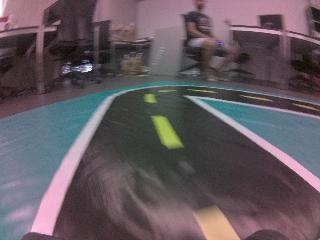
\includegraphics[height=0.50\textwidth]{experiments/11296.jpg}
  \end{minipage}%
  \begin{minipage}{.50\textwidth}
      \centering
      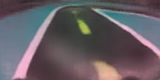
\includegraphics[width=0.60\textwidth]{experiments/11296.png}
  \end{minipage}
  \captionof{figure}{(Left) An image from the real world as seen by the DonkeyCar camera. (Right) The reconstructed image produced by the \textit{real VAE}.}
  \label{fig:realvaeexample}
% \end{figure}
% \begin{figure}
  \begin{minipage}{.50\textwidth}
    \centering
    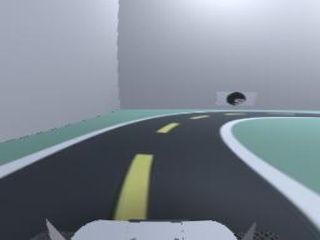
\includegraphics[height=0.50\textwidth]{experiments/1160.jpg}
  \end{minipage}%
  \begin{minipage}{.50\textwidth}
      \centering
      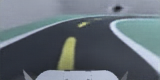
\includegraphics[width=0.60\textwidth]{experiments/1160.png}
  \end{minipage}
  \captionof{figure}{(Left) An image from the simulator as seen by the DonkeyCar camera. (Right) The reconstructed image produced by the \textit{simulated VAE}.}
  \label{fig:simvaeexample}
\end{figure}

\section{RL Algorithm}

\subsection{Reward Function}

Designing a reward function that is effective both in simulation and in the real world is challenging given the fundamental differences between simulated and real world environments. Indeed, in simulation, the environment can provide supervision and useful information such as the position of the car and the speed, that can be used to shape the reward function to guide the training. In our real setup, instead, the DonkeyCar can only leverage information coming from the camera. In particular, we consider the following reward function for both environments:

\begin{equation}
	\label{eq:realreward}
	r_t = 1 + \textit{throttle\_reward} + \left\{\begin{matrix}
		if \textit{done} & \textit{reward\_offtrack} \\ 
		else & 0  
	\end{matrix}\right.
\end{equation}

The first term is a constant bonus for each timestep, that encourages the agent to stay \textit{alive}, i.e. to stay on track in order not to abort the episode prematurely. The second term, i.e. \textit{throttle\_reward} $= (\textit{throttle} - \textit{min\_throttle}) / (\textit{max\_throttle} - \textit{min\_throttle})$, which encourages the agent to go as fast as possible. However, for simplicity and to reduce training time especially in the real world, we keep the throttle constant such that the second component is always zero. Finally, the agent receives a big negative reward (\textit{reward\_offtrack} $= -10$) when it goes offtrack. In simulation, this check is automated and corresponds to a cross-track error (XTE) greater than 3 (i.e., all the car is out of track with all four wheels), while in the real environment the episode is stopped manually when the car goes offtrack. Otherwise, when episode finishes without the car going offtrack (1000 timesteps pass since the beginning of the episode), the agent is not rewarded nor it gets a penalty.

%The reward function designed to work in simulation consists of four parts. The first one is a single point gained by the agent for every step made, intending to improve the length of the path as much as possible. Secondly, a throttle reward term increases the reward by a value proportional to the throttle to encourage the agent to drive as fast as possible. Moreover, a cross-track error penalty is proportional to the distance of the car from the center of the roadway that disincentives the agent as soon as it moves away from the center. Finally, as soon as the agent crashes or exceeds the maximum cross-track error allowed a big penalty is given. Thus, the reward function to be maximized is composed as follows:
%
%\begin{equation}
%  \label{eq:stdreward}
%    r_t = 1 + throttle\_reward + cte\_penalty + \left\{\begin{matrix}
%    if done & crash\_error \\ 
%    else & 0  
%    \end{matrix}\right.
%\end{equation}
%
%In our setup, the throttle is kept constant for the purposes of this thesis.
%The reward function described above is used to test our simulated algorithm and as a starting point, however, we need to adapt it such that it can work also in the real world where the cross-track error is not available. To tackle the issue we simply remove the CTE penalty, even though this will lead to a major problem of shaky motion as described in the next section. The final reward function that has proven to work in both environments and that we will use in the following training procedures is computed as follows:
%
%\begin{equation}
%  \label{eq:realreward}
%    r_t = 1 + throttle\_reward + \left\{\begin{matrix}
%    if done & crash\_error \\ 
%    else & 0  
%    \end{matrix}\right.
%\end{equation}
%
%Since we want real and simulated version of our agent as similar as possible, Equation \ref{eq:realreward} is finally used in both cases.

\subsection{Training the RL Agent in Simulation}

%As a baseline for our RL algorithm, we used the source code provided by \citet{learning-to-drive-in-5-minutes} as a baseline. His algorithm allows the training of many RL algorithms, including the SAC of our interest, of both simulated and real-world agents, however, training on simulation with communication being over the internet is more computationally expensive and more prone to errors. Thus, for the simulation, we refactor the algorithm such that the communication happens locally. Moreover, his algorithm uses an AE which needs to be changed with the more performant VAE chosen above. 

In simulation, we evaluated different \textit{reset strategies} in order to understand how the performance of the RL agent varies. In order to define the different reset strategies we rely on \textit{checkpoints} placed along the track (see Figure~\ref{fig:usitracksim}). In total there are seven checkpoints, distributed in this way: three of them are in the straight road, one checkpoint is in the middle of the first right curve and one at the end; then, there is another in the middle of the left curve and one at the end of the last but one right curve. \matteo{Maybe identify each checkpoint in the figure with a name.}

Based on such checkpoints we define the following reset strategies with various levels of human intervention, considering such strategies applied in the real world:

\begin{itemize}
	\item \textbf{Starting Line}: the agent always starts at the starting line when the episode starts. This is the default reset in the DonkeyCar Gym environment. The starting line is placed in the middle of the straight road sector of the track (see Figure~\ref{fig:usitracksim} and Figure~\ref{fig:usitrack}); 
	\item \textbf{Random}: the agent is placed in a random checkpoint every time an episode starts. The idea behind this strategy is to make the trained agent robust w.r.t. the starting point, since starting always from the same position (i.e., the Starting Line strategy) might lead the agent to repeat one sector of the track more often than the others;
	\item \textbf{Closest Checkpoint}: when the episode finishes the agent is placed to the closest checkpoint w.r.t. its position at the end of the episode;
	\item \textbf{All Checkpoints}: in this strategy we keep track of the latest checkpoint the agent was placed in the previous episode and we restart the next episode by placing the agent in the next checkpoint. Once all checkpoints have been \textit{covered}, we restart from the first.
\end{itemize}

If we had to rank such reset strategies by the manual effort required by the human operator when training the agent in the real world, we would rank Starting Line, Random and All Checkpoints in the top positions, since the operator would need to take the car and place it in a position that is potentially far from the position the car went offtrack. On the other hand, the Closest Checkpoint strategy would be the cheapest since the car would need to be placed closely to where it went offtrack.

For each reset strategy we trained a SAC agent by using the pretrained \textit{simulated VAE} trained earlier for 100\textit{k} timesteps, which corresponds to $\approx$ two hours of training on a MacBook without GPU. During training we track different metrics, i.e., the episode length, the episode reward and the success rate. Regarding the success rate, an episode is considered successful if the agent is able to return to the checkpoint it started from \matteo{check}. Figure~\ref{fig:agentresults} shows the results of the training process for the four agents. Each plot shows the respective metric averaged over 100 episodes. For example, each point in Figure~\ref{fig:agentresults}.a is the episode length averaged over the previous 100 episodes. 

%To train our agents, we need to define what is the best strategy in terms of the starting point. We identified four main options, the first one lets the Donkey start always at the starting line, the second option starts the Donkey from a random checkpoint, the third one at the latest checkpoint reached in the previous episode and finally, the last option makes it start from all checkpoints cyclically. Defining in simulation which is the best strategy can save computational time in real-world training. To identify which one eventually converges more quickly and if it does, 4 different agents were trained, one for each option aforementioned. The quality measures to evaluate the trained agents, illustrated below in Figure \ref{fig:agentresults}, are the \textit{Episode success rate} that shows how many laps have been completed on average during the training, the \textit{Episode Reward mean} and the \textit{Episode Length mean}. All the models have been trained for 100k iterations which correspond to $\approx 2$ hours of training. \textit{ Agent 1} started each lap at a random checkpoint,\textit{ Agent 2} started always at the starting line,\textit{ Agent 3} at the latest checkpoint reached during the last episode, and, finally,\textit{ Agent 4} cyclically uses all the checkpoints.

\matteo{Lines in Figure 5.3 are thin, I would make them thicker. Moreover, the yellow line is not visible; I would use another color.}

\begin{figure}[h]
  \centering
  \begin{subfigure}{.45\linewidth}
      \centering
      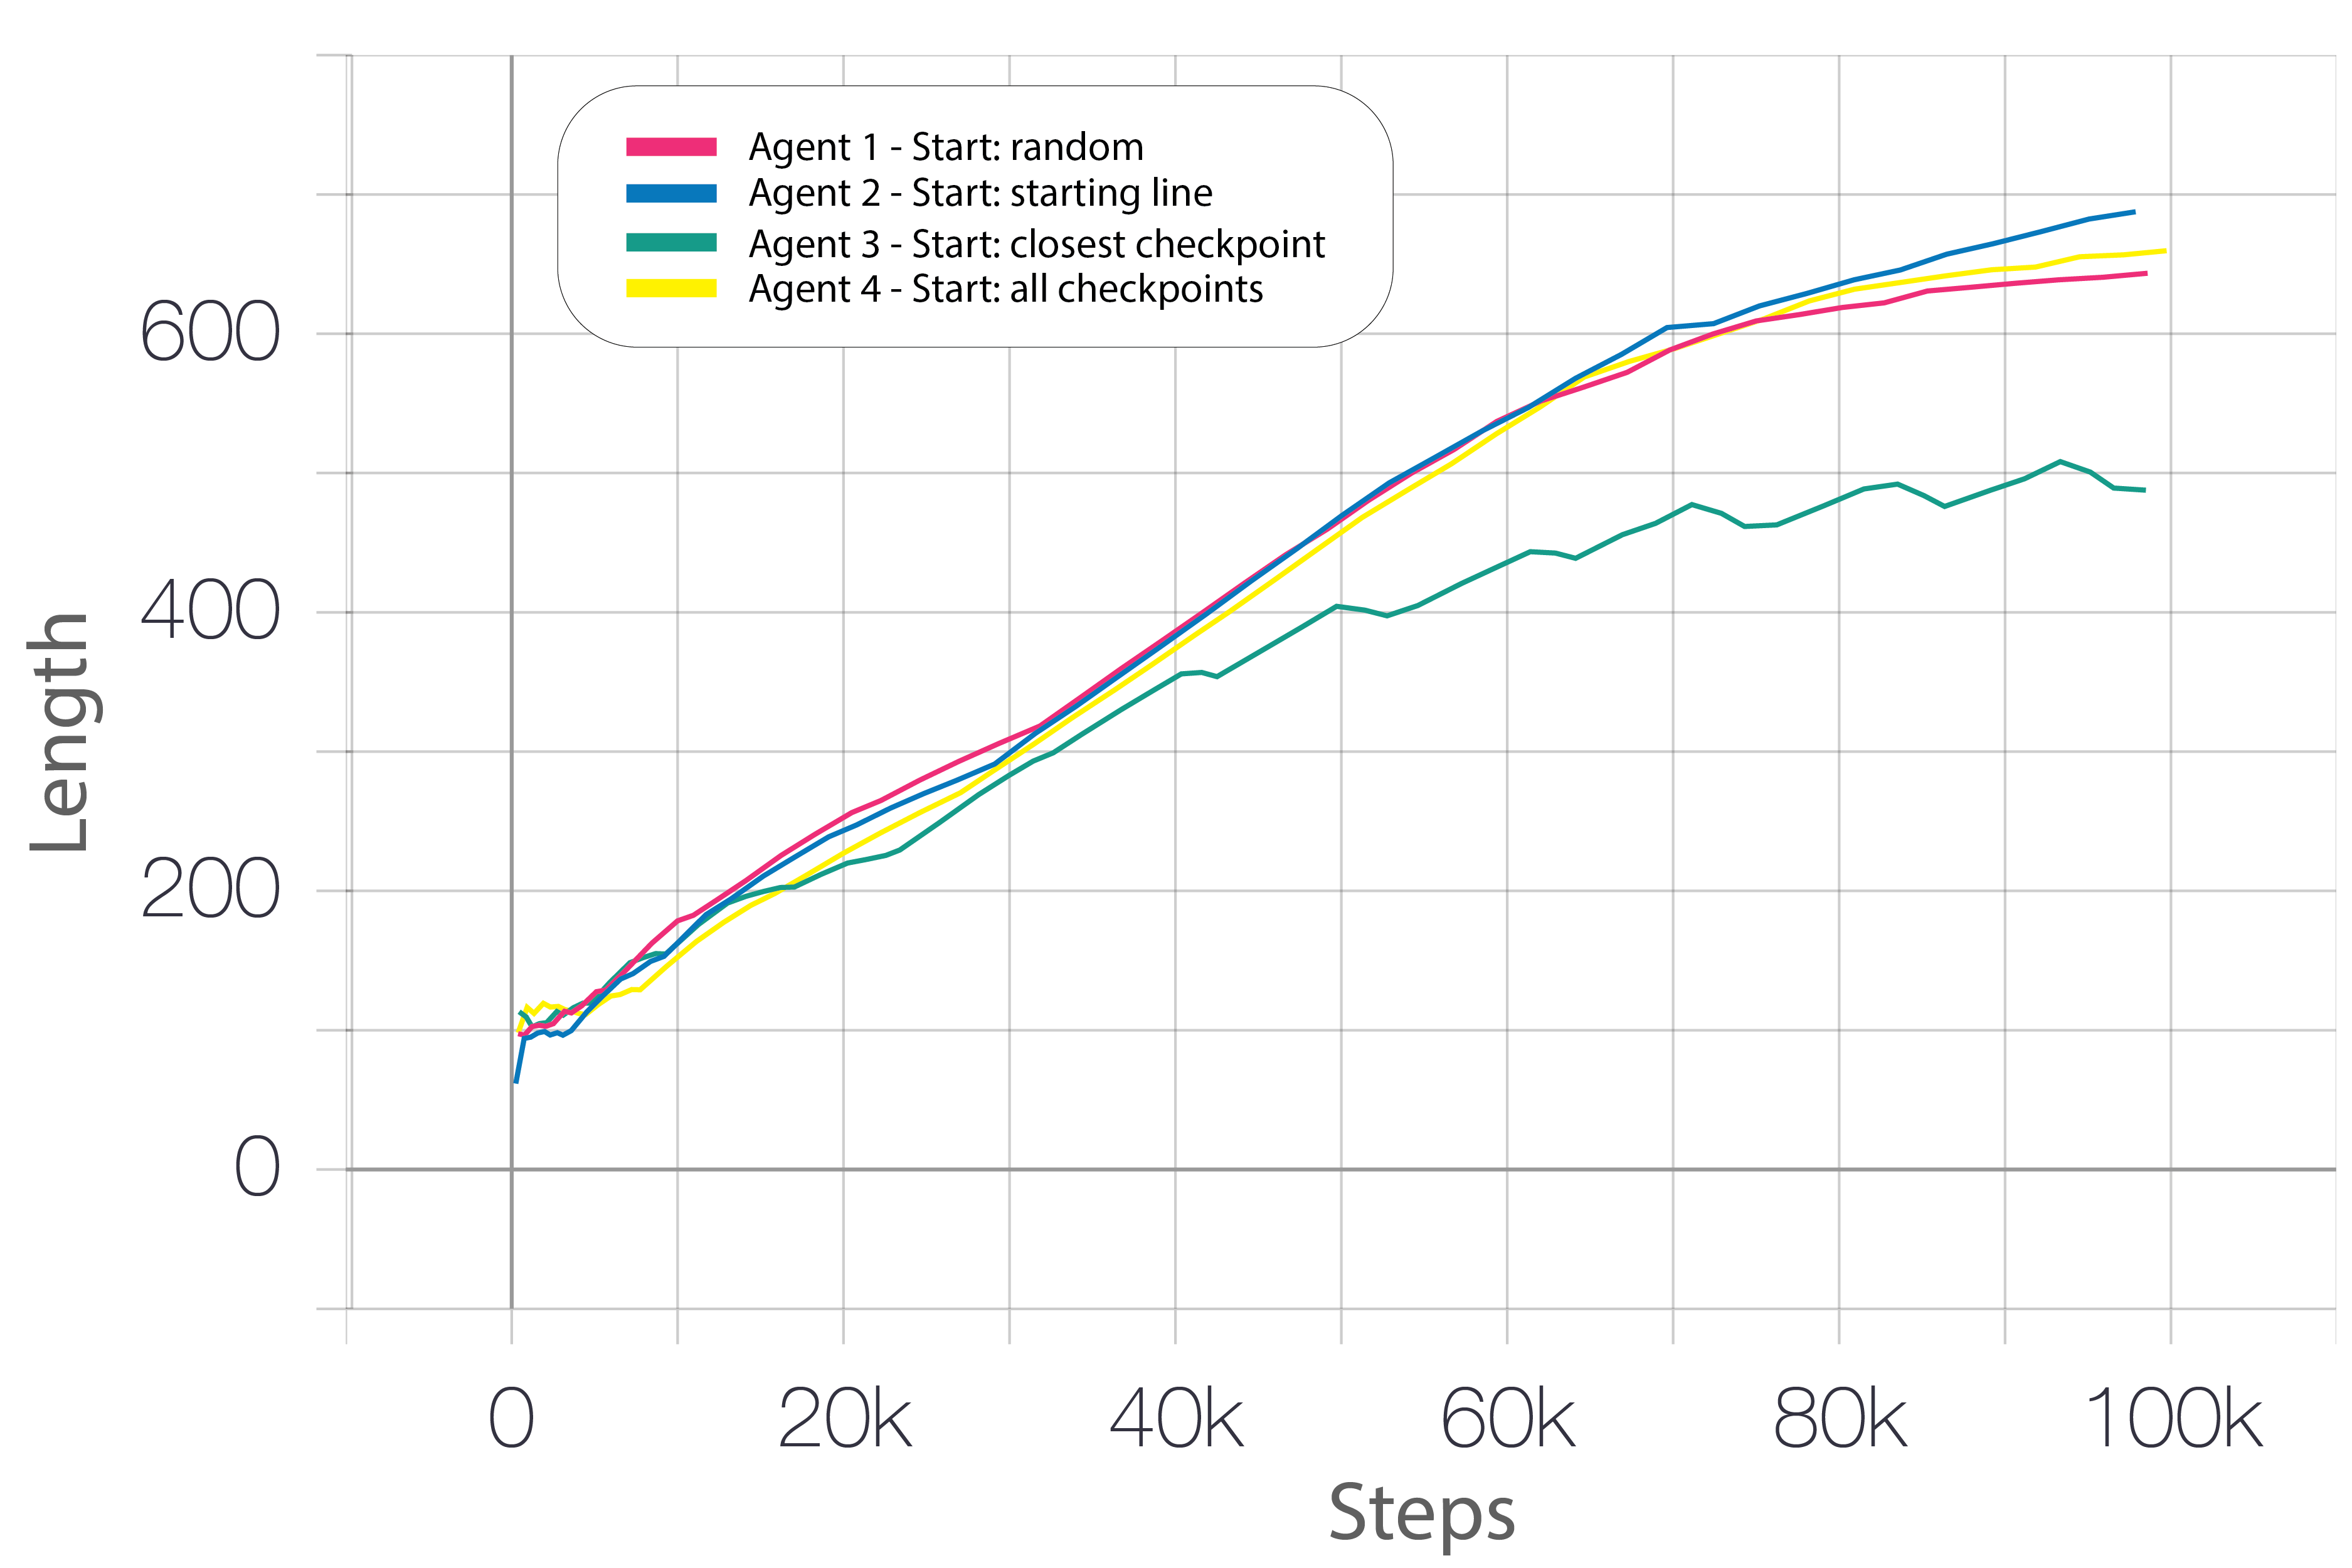
\includegraphics[width=1\textwidth]{experiments/len_mean.png}
      \caption{Mean episode length}\label{fig:len}
  \end{subfigure}%
      \hfill
  \begin{subfigure}{.45\linewidth}
      \centering
      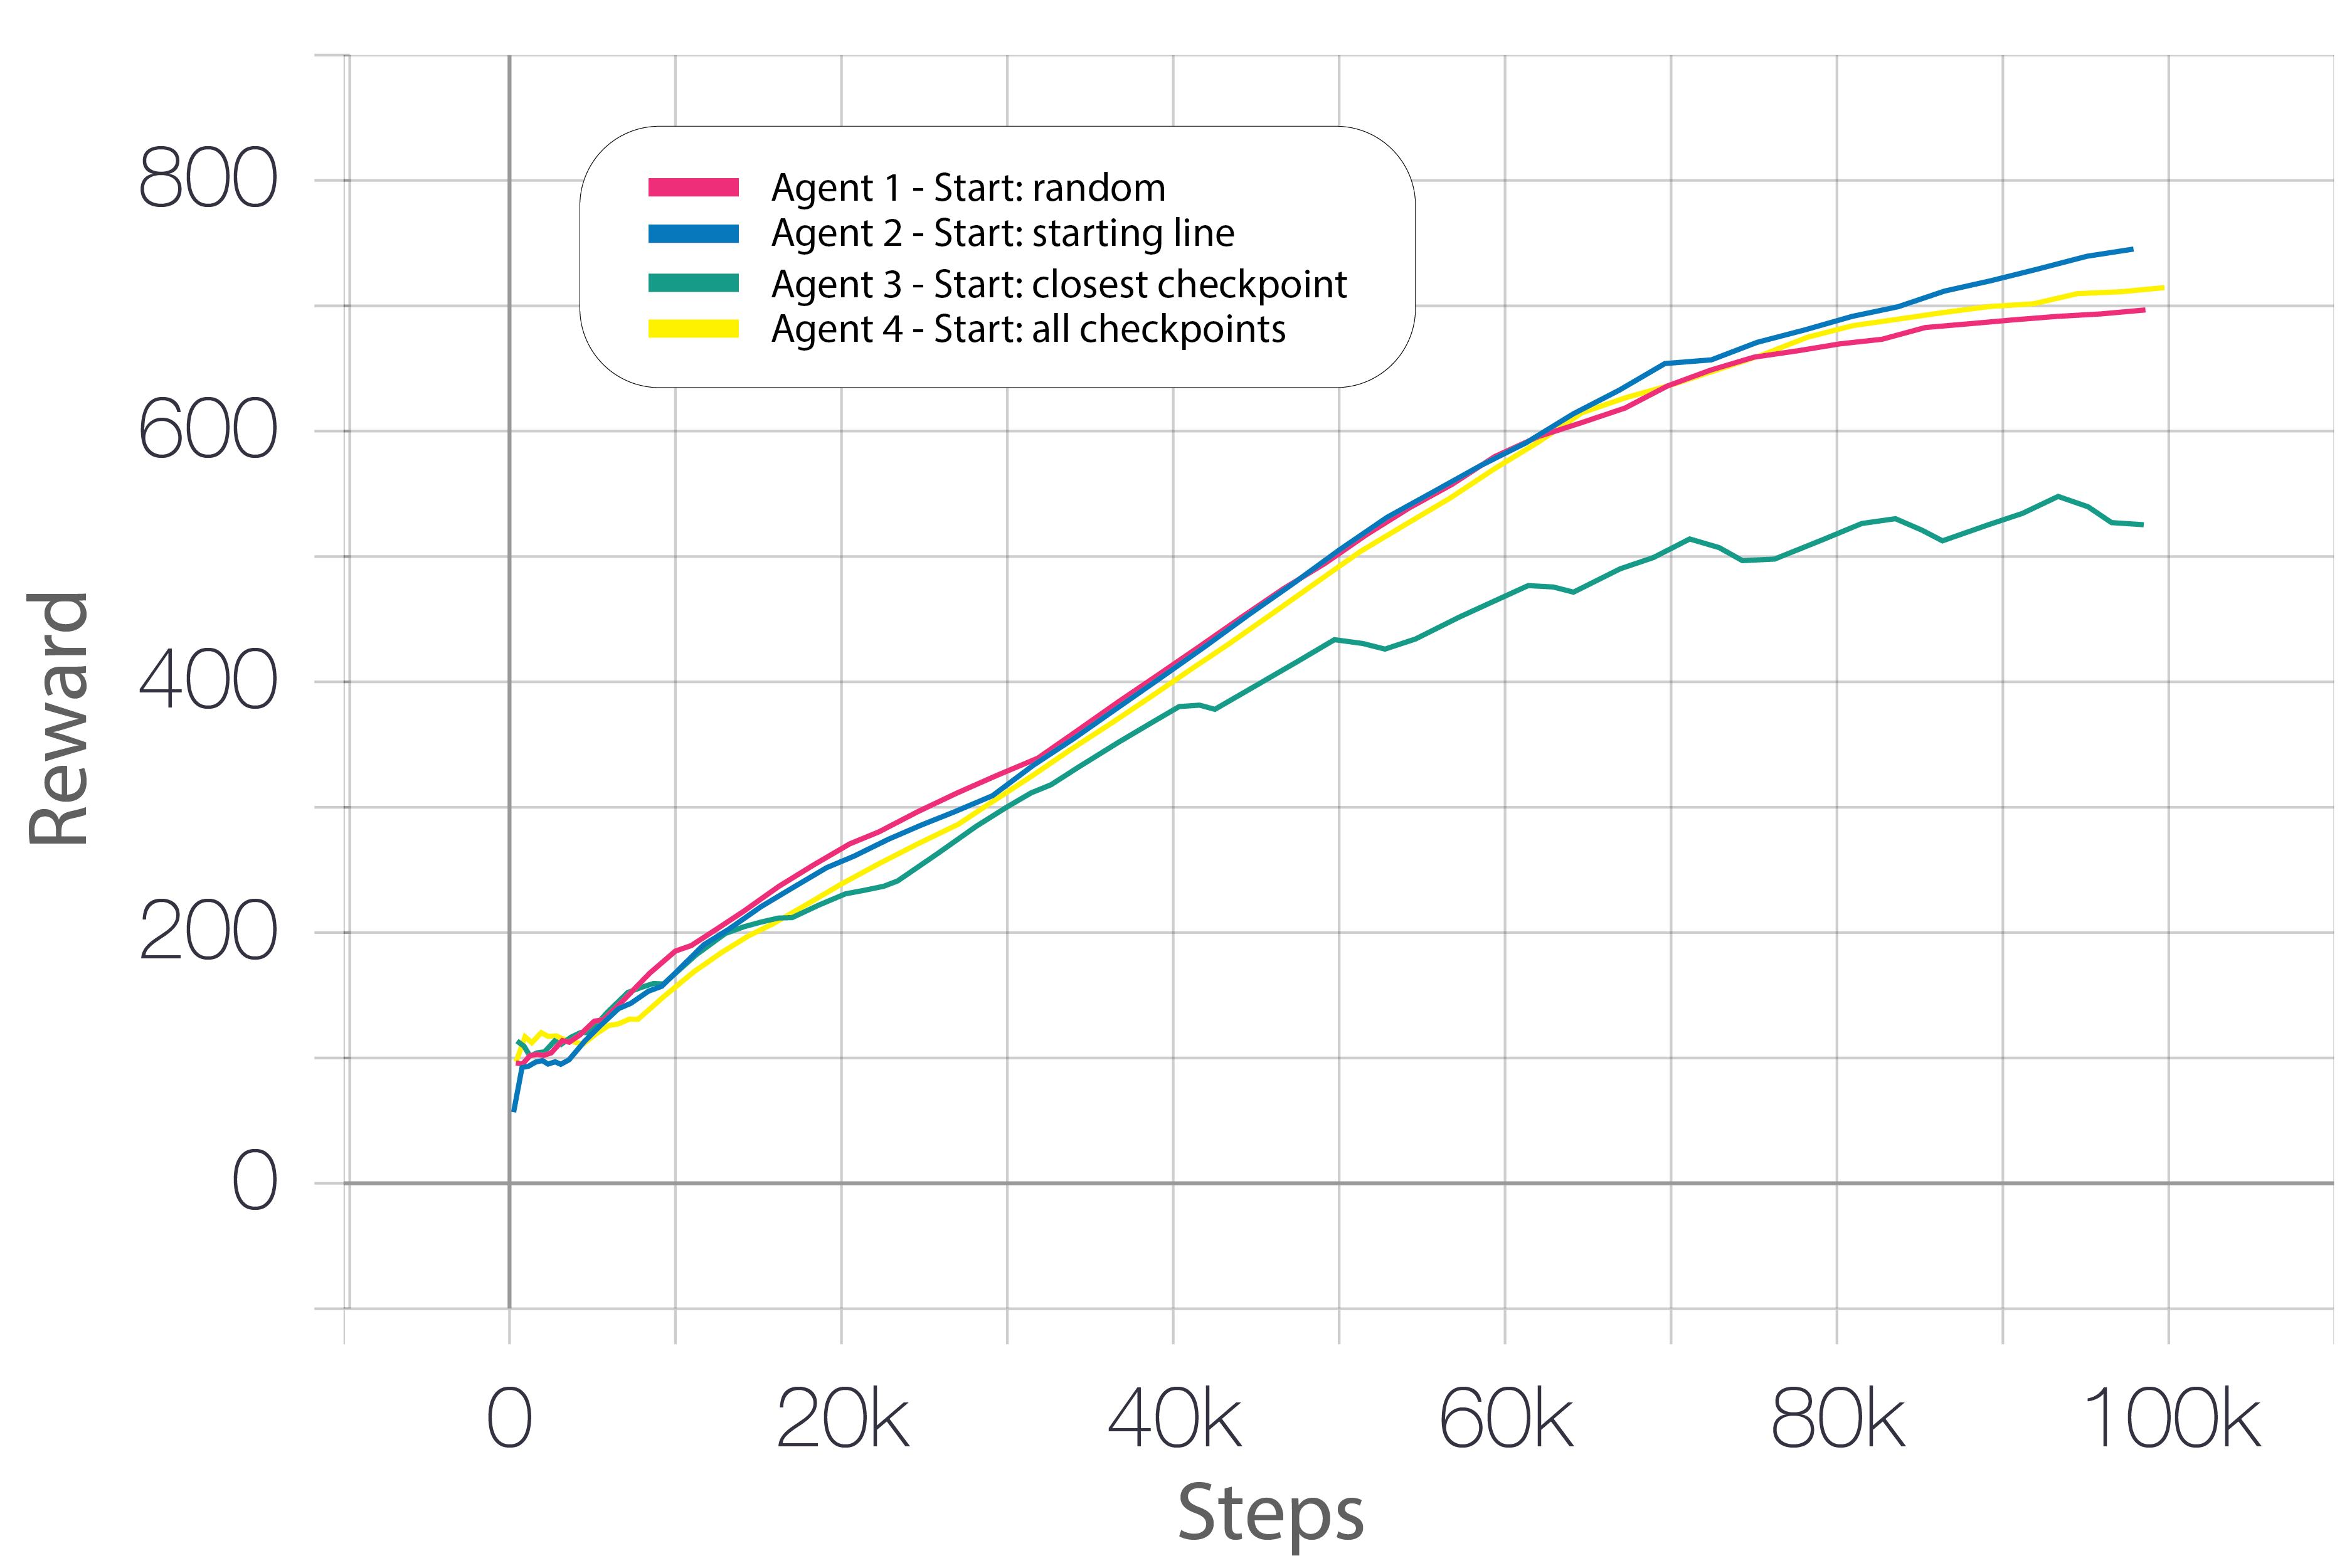
\includegraphics[width=1\textwidth]{experiments/rew_mean.png}
      \caption{Mean episode reward}\label{fig:rew}
  \end{subfigure}
  
  \bigskip
  \begin{subfigure}{.45\linewidth}
    \centering
    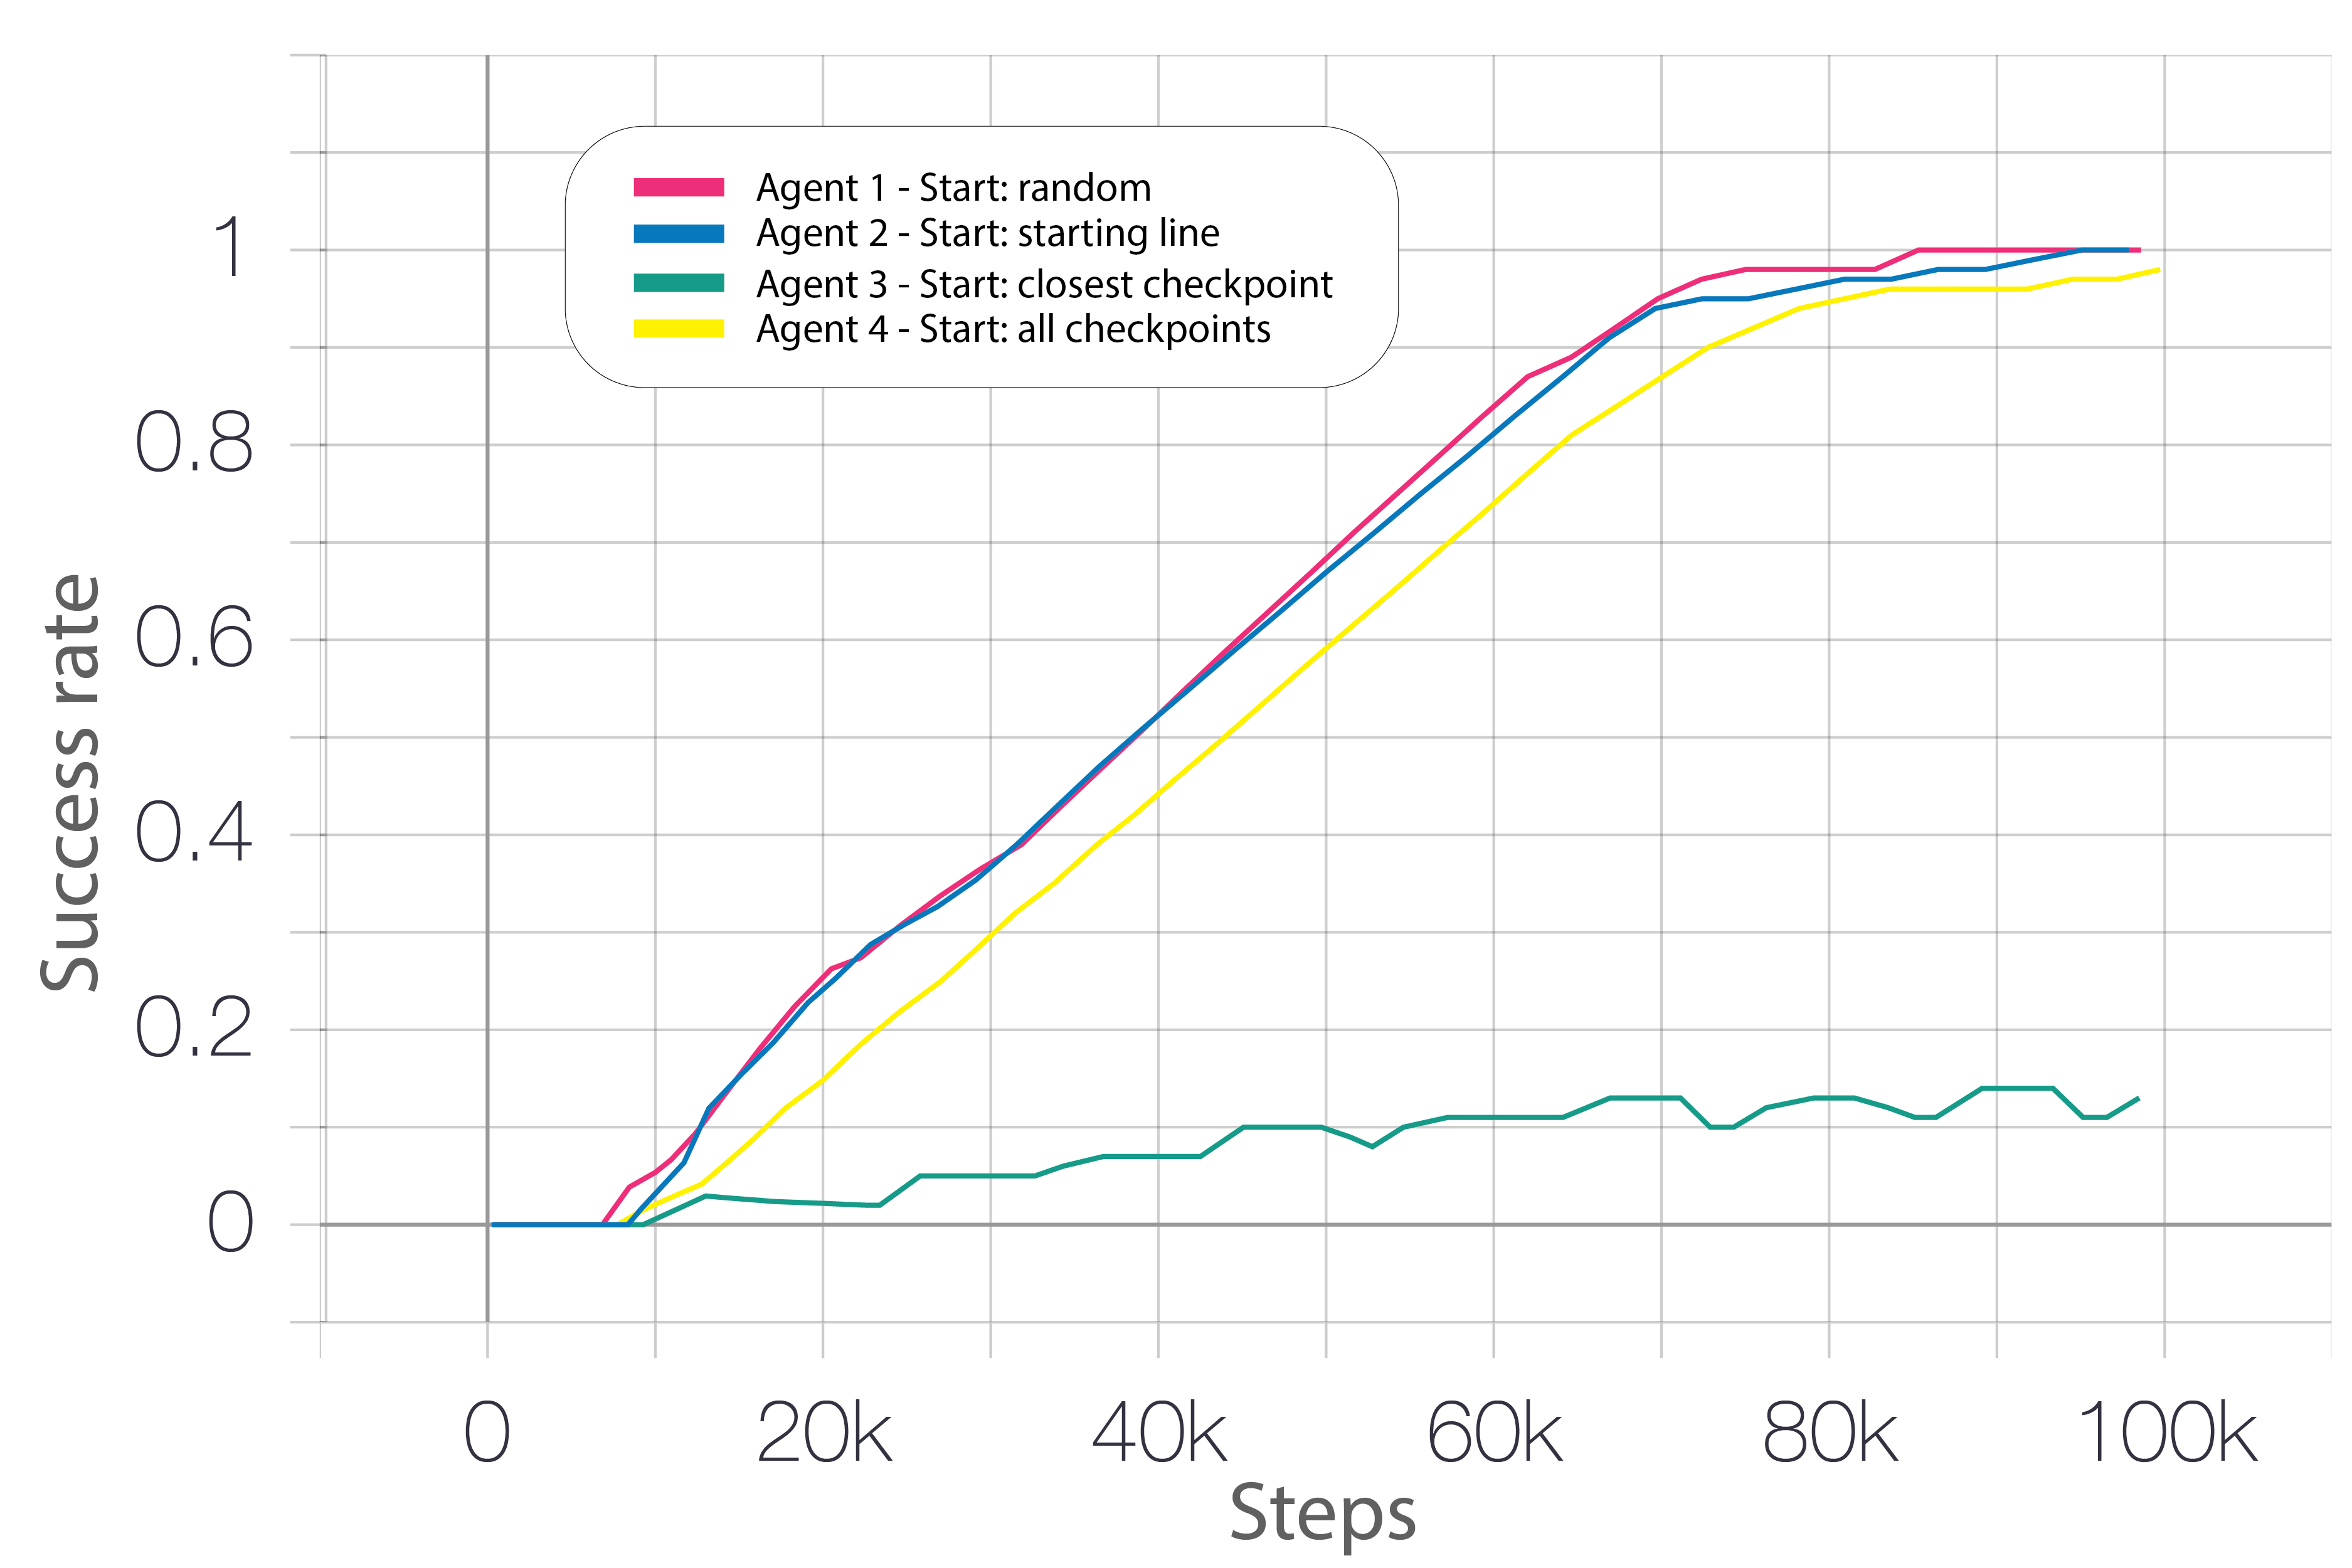
\includegraphics[width=1\textwidth]{experiments/success_mean.png}
    \caption{Mean success rate}\label{fig:succ}
  \end{subfigure} 
  \caption{Agents trained in simulation. Each agent has been trained with a different reset strategy for 100k steps.}
  \label{fig:agentresults}
\end{figure}

%During our experiments, we noted that, in the best case, a lap may take $\approx 350$ iterations to be completed. 

From the figure we can see that, for most strategies, the agent is able to reliably complete the task, except for the Latest Checkpoint strategy. The first two plots show the same trend for all agents; indeed, the reward function is directly linked to the episode length. Interestingly, although for the successful strategies the mean success rate converges at the end of training, which means that the agents are able to consistently finish the lap, the reward, and the episode length, keep increasing. The reason is that the agent is encouraged by the reward function to drive slowly while staying on track. Indeed, one way of slowing down is to learn a zig-zag trajectory, which is the way the agent learns to drive. 

Another interesting result is the one achieved by the Latest Checkpoint strategy. Indeed, following such reset strategy the agent is not able to learn how to drive around the track, achieving a negligible 10\% success rate. However, if we observe both the mean episode length and the mean episode reward plots (i.e. Figure~\ref{fig:agentresults}.a and Figure~\ref{fig:agentresults}.b) we can see that the respective value increases over time. In order to understand this particular behaviour, we took the trained agent and tested it on the same physical track. We observed that the agent found a \textit{blind-spot} where the simulator does not accurately measure the XTE. Figure~\ref{fig:bug} shows the sector in the track where the DonkeyCar goes offtrack (such position is close to the last but one right curve). Essentially, the agent goes offtrack in a position where the XTE is not accurately computed which means that the episode is not terminated and the agent is free of roaming in the scenario, without realizing being offtrack but accumulating reward points nonetheless. This behaviour can be observed only with this reset strategy. The reason is that, when the agent reaches the checkpoint before the last but one curve on the right, it cannot easily overcome the very challenging curve. Instead, it is easier for the agent to turn left in the exact positions where the XTE computation does not signal the end of an episode.

%The agents are all able to successfully learn to drive with a strict maximum CTE (3) except for \textit{Agent 4} which started new laps from the latest checkpoint. Two interesting shreds of evidence come out of those pieces of training. The first one is that even though the success rate mean approaches $100\%$, meaning the agents can consistently finish laps, the reward mean keeps growing. This shows a limitation in the reward function used, in fact, the agent gets a reward for every step and hence it learns to finish the lap following the longest path it has discovered. Moreover, the best way to lengthen the path is a zig-zag trajectory that allows also a doubling of the reward per lap. Secondly, the agent that starts at the latest checkpoint keeps improving the reward up to more than an equivalent completed lap, however, it never finishes a lap as described in Figure \ref{fig:succ}. 
%The reason behind this strange behavior is that the agent found a bug in the simulator used, as shown in Figure \ref{fig:bug}. Essentially, there is a little spot, off track, close to the steepest turn where the CTE is not correctly detected by the simulator, and consequently, the episode is not terminated. The reason why this behavior only happened with this agent lies in the training modality. When the agent reaches that checkpoint, he cannot easily reach the next checkpoint given the toughness of the turn, instead, it finds it easier to explore the bugged spot which is almost right in front of it when it approaches the turn.

\begin{figure}[h]
  \begin{center}
    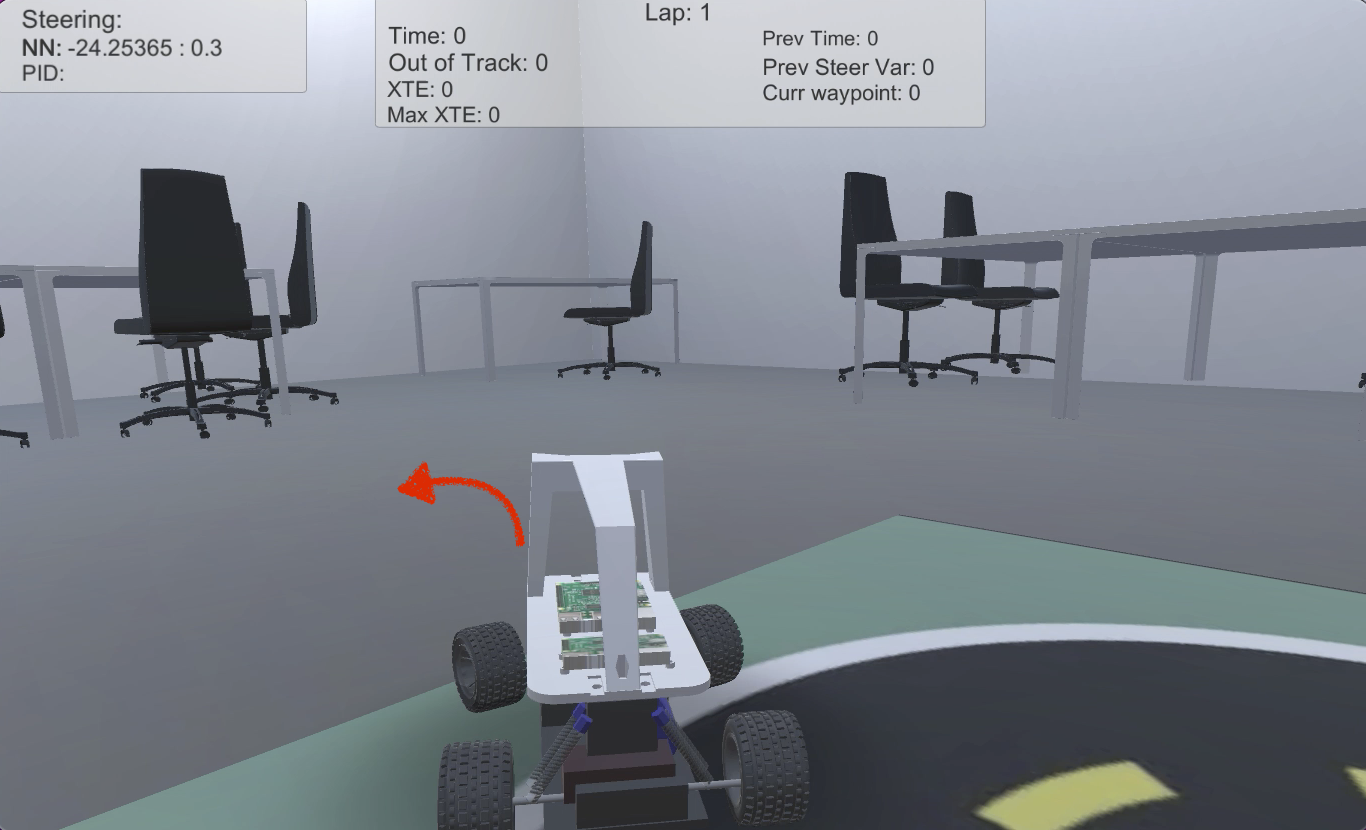
\includegraphics[width=0.50\textwidth]{experiments/bug.png}
  \end{center}
  \caption{Blind-spot in the simulator being exploited by the agent}
  \label{fig:bug}
\end{figure}

After training, we took the final agents for each reset strategy and tested them on the same track. In particular we executed each agent 10 times and enabled deterministic actions for the SAC algorithm, which means that, given an observation, the trained stochastic policy selects the action with the highest probability. Indeed, we executed each agent multiple times to account for the randomness of the simulator. A lap is successful when the car is able to return to the starting checkpoint according to the reset strategy \matteo{check}. The results of such experiments are shown in Table~\ref{tab:simagent}.

%To further test the trained agents, for 10 laps it is measured how many times a lap has been completed by each agent, how many times the agents crash, and finally how many times they exceed the roadway but can recover and finish the lap without crashing. The result are presented in Table \ref{tab:simagent}.

\begin{table}
  \centering
  \begin{tabular}{|c|c|c|c|c|c|}
  \hline
  AGENT & \# OOT & \# OBE & SUCCESS RATE & MEAN EP. LENGTH & MEAN EP. REWARD \\ \hline
  1 (R) & 0 & 0 & 1 & 595 & 644 \\
  2 (SL) & 0 & 4 & 1 & 599 & 647  \\ \hline
  3 (AC) & 0 & 0 & 1 & 624 & 676 \\
  4 (CC) & 10 & 29 & 0 & 460 & 495  \\ \hline
  \end{tabular}
  \caption{Agents results averaged over 10 runs. \matteo{In the plots Agent 4 is the one trained with AC while here it is the one trained with CC.}}
  \label{tab:simagent}
\end{table}

During testing we measure the average Out of Track (OOT) events (second column), i.e., the number of times the agent goes offtrack, the average Out of Bound (OOB) events (third column), i.e., the number of times the measured XTE is greater than 2, the average success rate (fourth column) and the average episode length and episode reward (respectively fifth and sixth columns). An OBE event means that the agent momentarily exists from the roadway but it is able to recover. From the results we can see that all agents, except the agent trained with the Closest Checkpoint strategy, are able to successfully complete the ten laps. Since the average reward is comparable across the successful strategy, no clear winner reset strategy to be used in the real world training emerges.

%From the results is evident, excluding \textit{Agent 4} because of the simulator's bug, that three agents learned to successfully drive and in most cases, they always stay entirely on track without the need for any additional sensor and with the only problem of the shaky driving which is still acceptable for the purposes of this thesis, in most cases, they never get out of the track, and if they do they can recover consistently.

\subsection{Training the RL Agent in The Real World}

Since no clear winner among the reset strategies emerged from the experiments in simulation, all the reset strategies, including the Closest Checkpoint one, are viable to be tested in the real world. However, we only experimented with the default reset strategy, i.e. the Starting Line strategy, and the most convenient strategy in terms of supervision effort, i.e. the Closest Checkpoint strategy. Indeed, we trained two agents, i.e., one for each strategy, with the SAC algorithm and by using the pretrained \textit{real VAE}. Each agent was trained for $\approx$ 30 minutes.

\begin{figure}[h]
	\centering
	\begin{subfigure}{.5\linewidth}
		\centering
		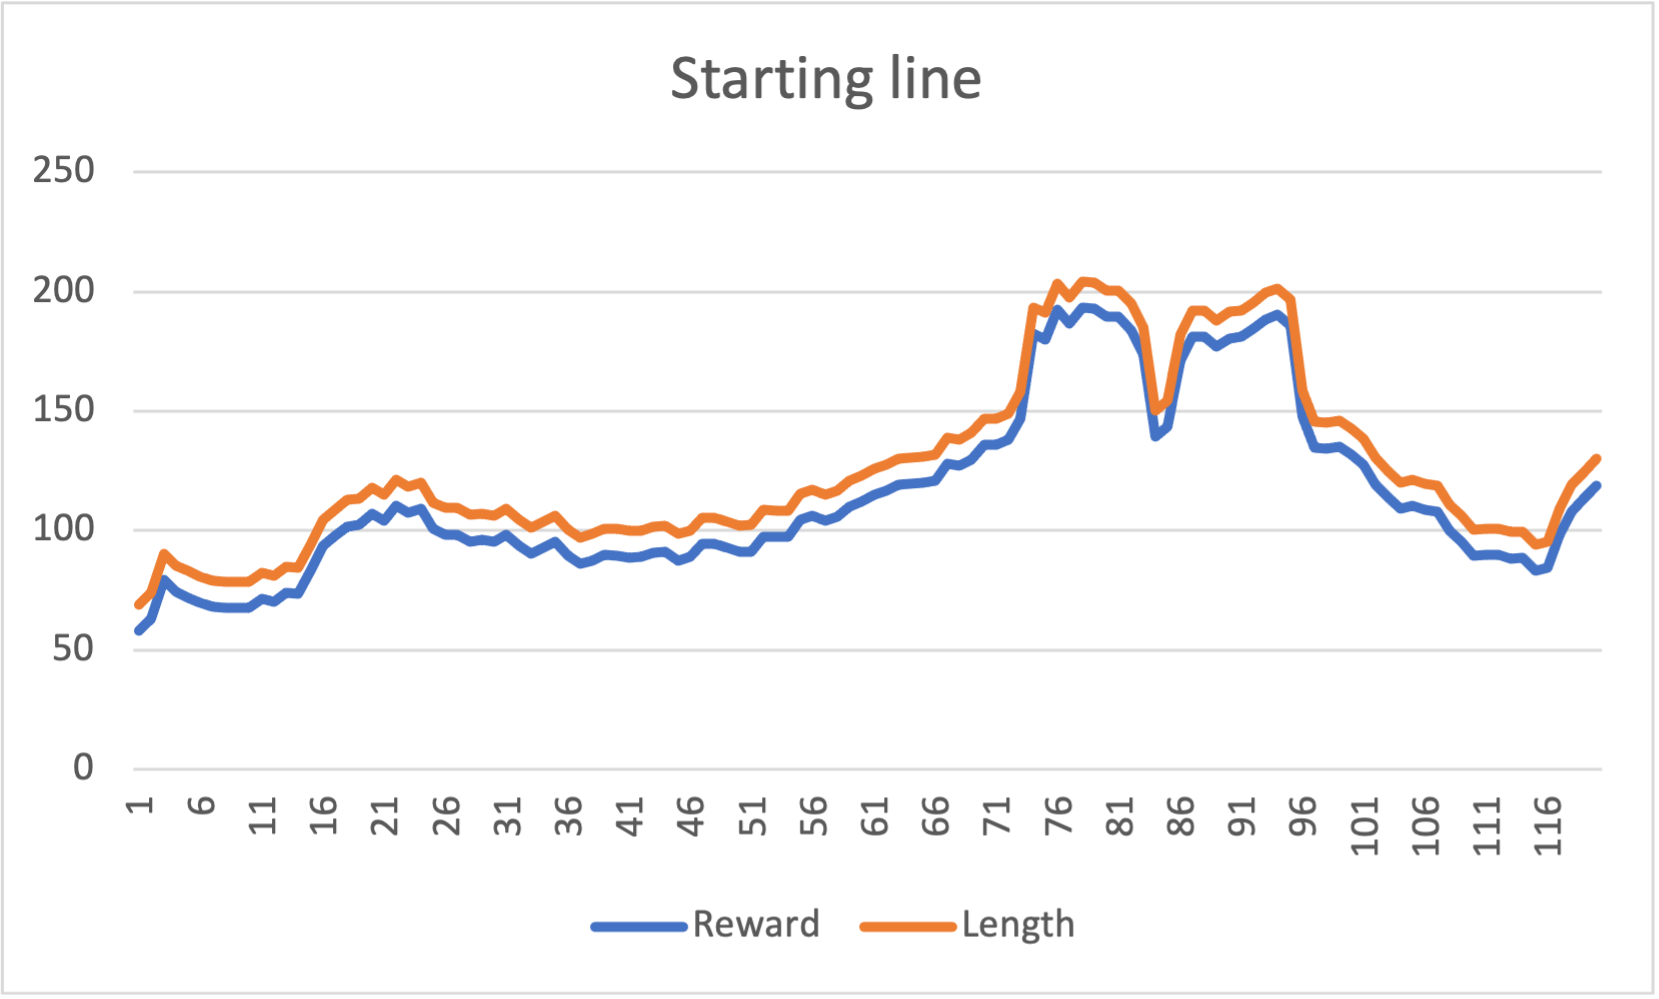
\includegraphics[width=1\textwidth]{experiments/badrealagentstart.png}
		\caption{Mean episode length and reward: Starting Line strategy}\label{fig:rlen}
	\end{subfigure}%
	\hfill
	\begin{subfigure}{.5\linewidth}
		\centering
		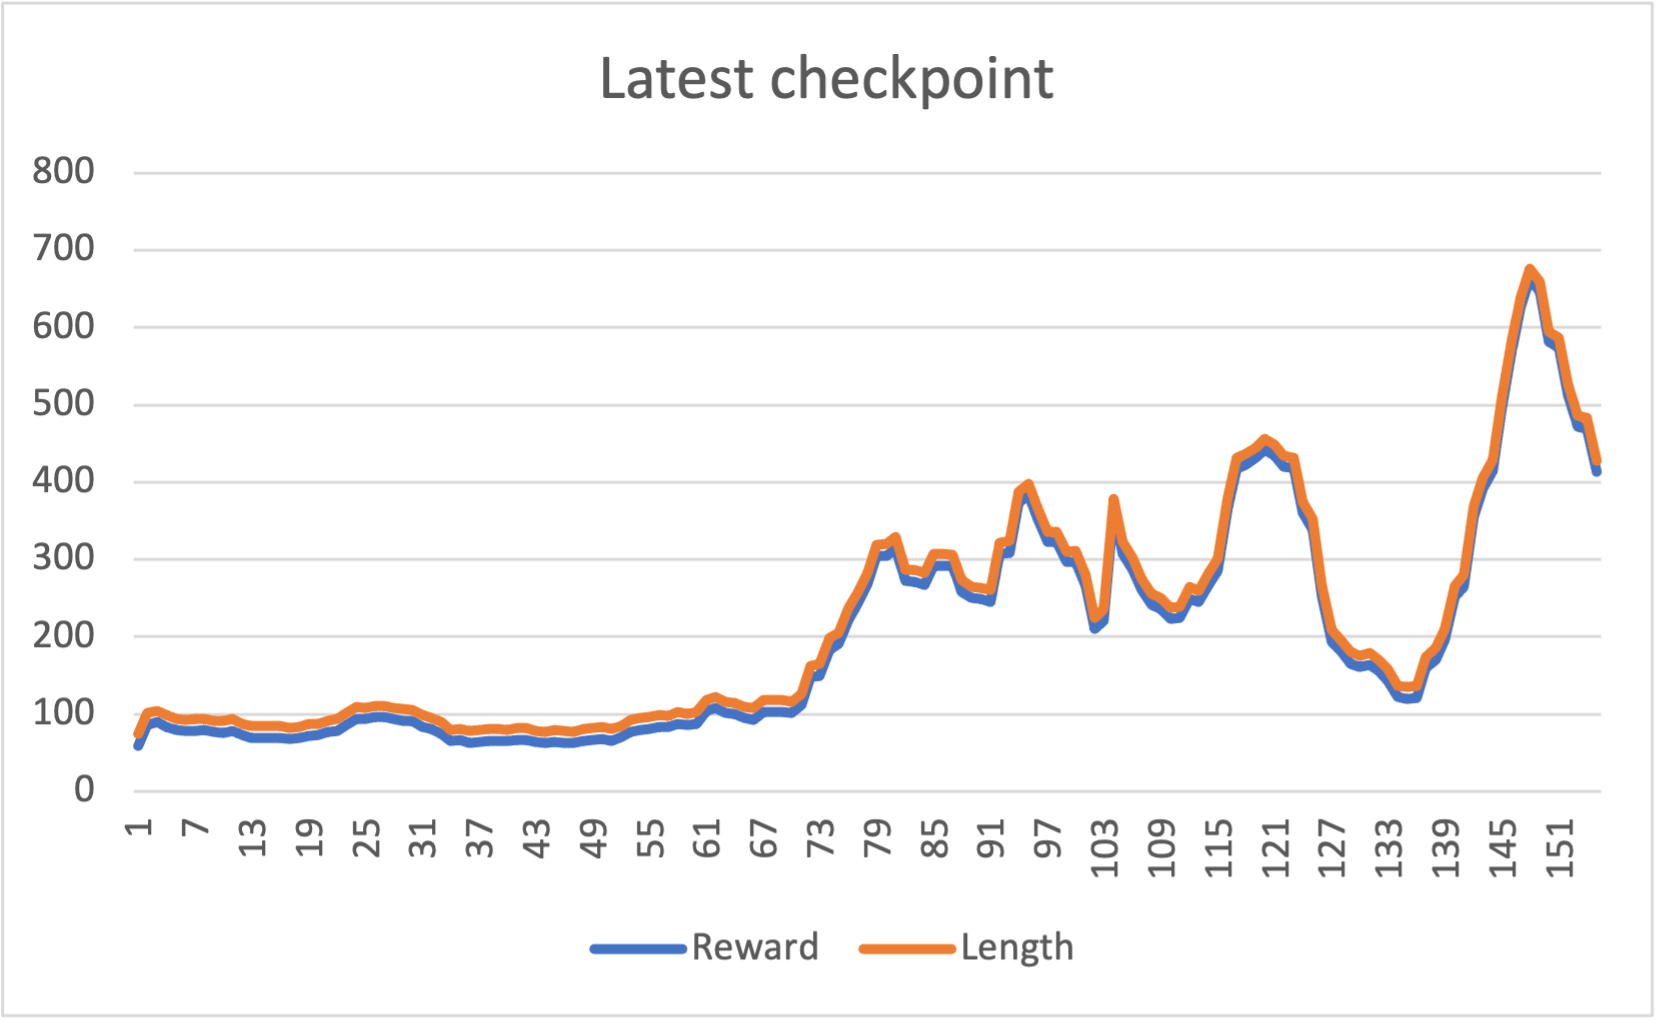
\includegraphics[width=1\textwidth]{experiments/badrealagentlatest.png}
		\caption{Mean episode length and reward: Closest Checkpoint strategy}\label{fig:rrew}
	\end{subfigure}
	\caption{Agents trained in real world with the Starting Line strategy (left) and Closest Checkpoint strategy (right). \matteo{Plots are not in scale ($y$-axis different), difficult to compare the results.}}
	\label{fig:realresult}
\end{figure}

Figure~\ref{fig:rlen} shows the training curves for the two agents. The two lines (i.e., $y$-axis) for each plot show the mean reward and the mean episode length across the previous 100 episodes \matteo{check}, while the $x$-axis shows the number of episodes, i.e., the training time.

From the plots we can see that the agent that learns with the Starting Line strategy did not manage to achieve a good reward given a budget of $\approx$ 100 episodes. On the other hand the other agent with the Closest Checkpoint strategy was able to achieve 100\% more reward with the same budget (i.e., 400 average reward vs 200 average reward). Therefore, after 100 episodes we decided to stop the training of the first agent, in order to save time. Instead, we carried out the training of the most promising agent, in order to observe further improvement. In total, such agent was trained for 45 minutes, taking approximately 30 minutes to complete a lap and by the end it was able to complete two laps (notice that in the real world an episode terminate successfully when 1000 timesteps pass, which correspond to $\approx$ 2.5 laps).

Interestingly, in the right plot of Figure~\ref{fig:rlen} both the average reward and the episode length show an oscillating behaviour starting at episode 73. Such behaviour can be explained by the different levels of difficulty of the track and by the reset strategy. Indeed, when the agent is placed at the starting line it is able to drive well since the initial part of the track is relatively easy to drive, with a straight line and a smooth right curve. Then, when the agent arrives in the challenging sectors of the track \matteo{which one?}, the agent goes offtrack and restarts in the closest checkpoint. Then, it takes the agent some time to learn how to drive in the challenging part and, as a consequence, the average reward decreases. The reward keeps decreasing until the challenging part is overcome and the it starts increasing again. This oscillating behaviour repeats multiple times during training until the agent is able to drive the challenging part at full speed.

Regarding the difference w.r.t. the Starting Line strategy we suspect that the advantage of the Closest Checkpoint strategy is that, in the latter, the agent is given the chance to learn the challenging part of the track at a low speed, since the agent starts close to it. On the other hand, if the agent always starts at the Starting Line, it is forced to learn the challenging part at full speed, which requires more training time.

To summarize, we were able to train a RL agent in the real world in a reasonable amount of time, i.e. $\approx$ 30 to 45 minutes, by decoupling state learning, which we addressed with a VAE, from policy learning which we tackled with the SAC algorithm. Moreover, we used a custom reset strategy that enabled training of an effective policy.

%To train the real-world agent, instead, the source code provided by \citet{learning-to-drive-in-5-minutes} is kept untouched beside the encoder, with the main goal being to replicate their results but with a more performing VAE as resulted in our tests. Given that in the real world the simulator's supervision is not available, all the strategies tested in the previous section are good candidates to be used, also \textit{Agent 4} strategy that cannot explore anymore the simulator's bug. In fact, in the real world, we only have human supervision that is about stopping the episode as soon as the car exceeds the track boundaries with all 4 wheels, while the server automatically stops the car when it reaches 1000 steps ($\approx 2.5$ laps). From the tests resulted that all the agents, trained with the aforementioned strategies, struggle to learn to drive an entire lap, at least in a reasonable time, except\textit{ Agent 4 }that start his laps at the latest checkpoint reached in the last episode. For the sake of brevity, since they are all equivalent among the failing agents, only the results of the agent that starts always at starting line and fails in learning, as shown in Figure \ref{fig:rlen}.
%
%In figure \ref{fig:rrew}, instead, are shown the performances in the training of the agent starting at the latest checkpoint (equivalent strategy of previous \textit{Agent 4}), which can be considered successful and comparable to simulated agents since it did learn to complete a lap in about 30 minutes and two laps in about 45 minutes. In five to twenty episodes, the first two turns were learned decently and most of the time was spent on the steepest turn. As shown in Figure \ref{fig:rlen}, the graph is characterized by ups and downs, as soon as the car started at the starting line, it learned quickly, then, when the steepest curve was reached it struggled to overcome it and when it eventually did, the length started to increase again. The process was repeated until it was almost consistently able to finish a lap. Furthermore, as soon as the agent learned the steepest turn, it did generalize well on the following turns and little time was spent on them.
%
%Notice that the laying of the car at the latest checkpoint has been intentionally approximate on the area close to the checkpoints. This brought a main advantage, the agent learned quicker since it was able to see the area in front of it from many points of view and this, resulted useful when the car started to cross many checkpoints per episode since the direction from which the car arrived to a checkpoint could vary a lot, it had been trained to drive on many possible trajectories and was able to join the various sections well. Unfortunately, in the real world, more metrics to measure the quality of the driving and to make comparisons with the simulated agents are not available. 

\section{Sim to Real and Real to Sim}

In this section we present an unsuccessful attempt at transferring the agent trained in the real world in simulation (real2sim, or r2s for short). This transfer would be useful in order to better evaluate the real world agent, given the constraints of the physical world. Indeed, in simulation it is possible to generate tracks with any shape and length to test the capabilities of the given agent. Likewise, transferring an agent trained in simulation into the real world (sim2real or s2r for short), would be useful to automate the training process, especially in the reset, and avoid unsafe behaviour of the agent.

%Could not work also because we are only bridging the visual gap, while the physical gap is not addressed (see robot paper cited in testing-rl).

%In this section we present an unsuccessful attempt in driving our simulated DonkeyCar with the real agent trained above. SimToReal (S2R) and vice-versa aims in deploying model trained in one environment to the other. In our case, since the real world environment, in our setup, does not provide enough metrics to benchmark our real world agent, we aim to make it works also in simulation. For example, in order to test the generalization of the real agent would be much easier in simulation where multiple tracks or obstacles can be implemented at a low cost. Another advantage brought by this approach is that an agent trained in simulation, can be moved into the real world and this would result in less expensive training procedures and eventually more robust agents. 

We follow previous work~\cite{stocco-mind} that attempts to bridge the visual gap between simulation and real using image-to-image translation techniques. In particular, we train a CycleGAN~\cite{CycleGAN2017} to translate the images in one domain (real) into the other (simulated) and viceversa. In particular, we used the same hyperparameters of the original paper and trained the CycleGAN architecture for XX epochs \matteo{check}. During training we saved different checkpoints, we visually assessed the quality of the translations for some of them and picked the one with the best-looking translations. Figure~\ref{fig:cycleganexample} shows an example of translations generated by the CycleGAN generators (respectively, s2r generator in Figure~\ref{fig:cycleganexample}.a and r2s generator in Figure~\ref{fig:cycleganexample}.b). The images generated by the CycleGAN generator are called \textit{pseudo}-real or \textit{pseudo}-simulated, since they are translations from one domain into the other.

%The idea is to pre-train a CycleGan \citep{CycleGAN2017} for image transfiguration. In fact, the CycleGan is able to move an image into another domain keeping the original structure unaltered, but applying the style of the other domain as shown in Figure \ref{fig:cycleganexample}. Thus we leverage this property to transform images seen by the simulated camera of the DonkeyCar into what it would see in real world and vice-versa. Then, a real agent will eventually be able to drive on the simulator since it does see pseudo-real images. On the other hand, in order to drive a real car with a simulated agent, our DonkeyCar has not enough computational power, hence it could not run in time a CycleGan, that has millions of parameters, to make the real car see pseudo-simulated images and drive with the simulated agent. However, the problem can be circumvented by training an agent entirely on simulation but with pseudo-real images. After training CycleGAN with our datasets, it is able to transfigure image with high fidelity as shown in Figure \ref{fig:cycleganexample}. In fact, in human eyes they are barely distinguishable. However, even if the result looks good it could not be the case for the AutoEncoder that needs to place similar real and pseudo real images close into the latent space and similarly for similar simulated and pseudo simulated images.

\begin{figure}[h]
  \centering
  \begin{subfigure}{.6\linewidth}
      \centering
      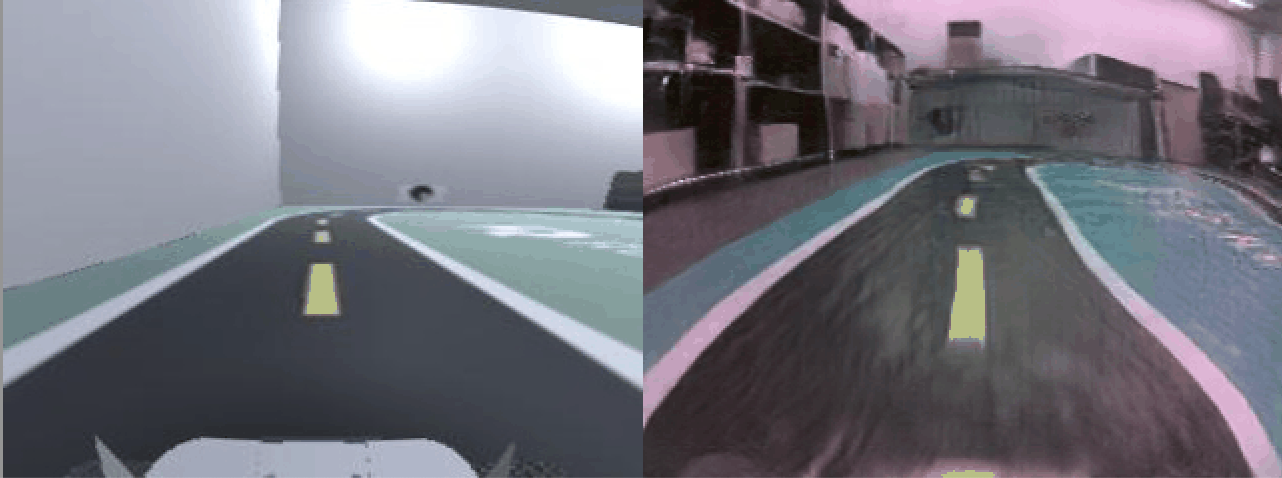
\includegraphics[width=1\textwidth]{experiments/s2r.png}
      \caption{From simulated images to pseudo-real.}\label{fig:s2r}
  \end{subfigure}
      \hfill
  \begin{subfigure}{.6\linewidth}
      \centering
      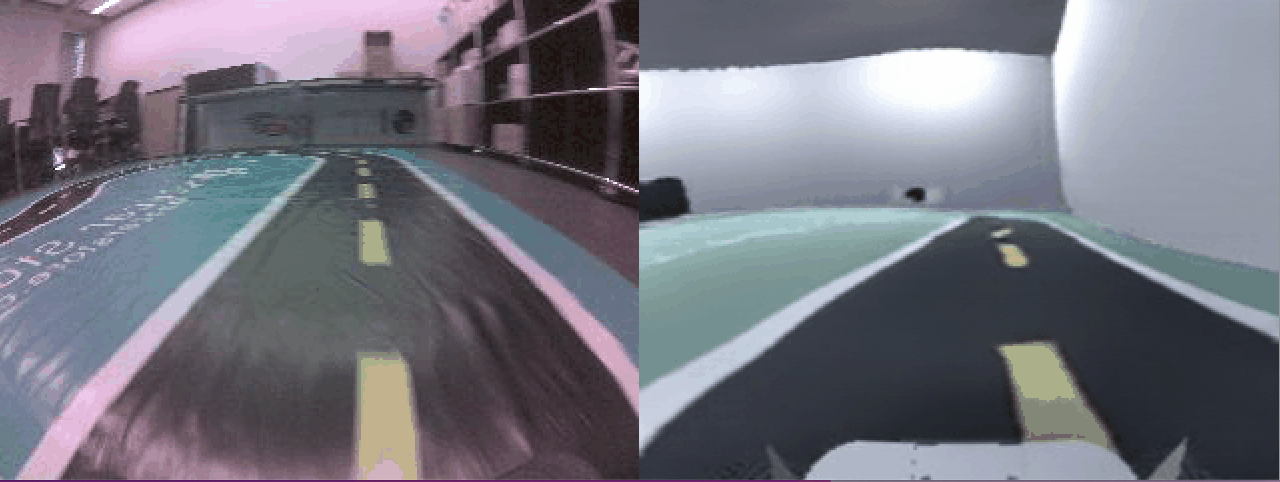
\includegraphics[width=1\textwidth]{experiments/r2s.png}
      \caption{From real images to pseudo-simulated.}\label{fig:r2s}
  \end{subfigure}
  \caption{Translations generated by the trained CycleGAN.}
  \label{fig:cycleganexample}
\end{figure}

Once the CycleGAN architecture was trained, we used it to translate the two test sets of images we collected to evaluate the \textit{simulated VAE} and the \textit{real VAE}. The objective of this preliminary analysis is to understand how the \textit{pseudo} images generated by the CycleGAN are mapped by the chosen VAEs in the two domains w.r.t. the \textit{authentic} (i.e., real and simulated images captured by the camera of the car) images. Indeed, if we want to use the CycleGAN to transfer the trained agent from one domain into the other, we have to translate each image coming from the camera into a pseudo image of the other domain, which is mapped by the VAE into the latent space; only then, the corresponding latent space is processed by the trained policy.

After translating the two test sets we computed the latent space for each image using the two VAEs and then applied the t-SNE dimensionality reduction technique~\cite{tsne} to visualize how the translations are mapped by the encoders w.r.t. the authentic images. The visualization is shown in Figure~\ref{fig:latentpseudo}.

\begin{figure}[h]
  \centering
  \begin{subfigure}{.5\linewidth}
	      \centering
	      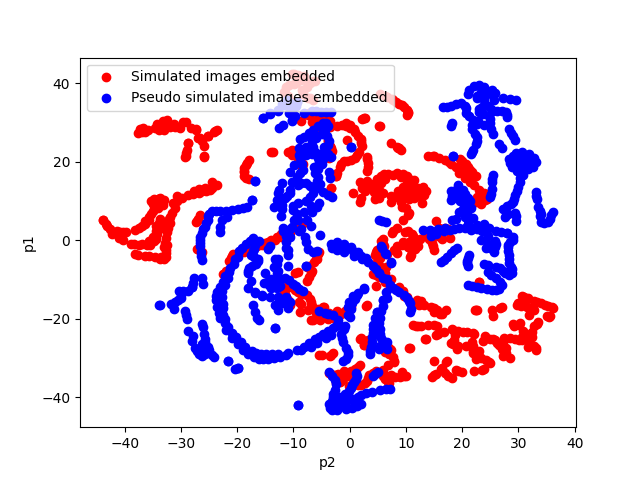
\includegraphics[width=1\textwidth]{experiments/latentr2s.png}
	      \caption{Simulated (authentic) and pseudo-simulated images}\label{fig:latentr2s}
	  \end{subfigure}%
      \hfill
  \begin{subfigure}{.5\linewidth}
	      \centering
	      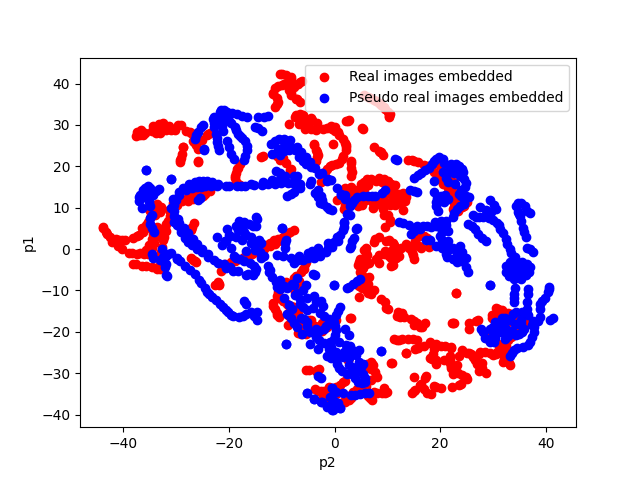
\includegraphics[width=1\textwidth]{experiments/latents2r.png}
	      \caption{Real (authentic) and pseudo-real images}\label{fig:latents2r}
	  \end{subfigure}
  \caption{Latent space visualization: authentic vs pseudo (i.e., translated) images. (Left) simulated VAE, (right) real VAE.}
  \label{fig:latentpseudo}
\end{figure}

Notice that the two test sets are not \textit{paired}. Indeed, both represent images of a lap taken by driving manually along the track in simulation and in the real world. However, despite the images should represent similar situations during driving, we can see that the embeddings do not consistently overlap, both in the r2s case (Figure~\ref{fig:latentpseudo}.a) and in the s2r case (Figure~\ref{fig:latentpseudo}.b). There are some regions, more prevalent in the s2r case, in which the embeddings produced by the VAE overlap for the pseudo and the authentic images, but there are others that are mapped in different regions. This could lead to the trained agent not to act consistently when presented with authentic and pseudo image, since the latent space that will be produced by the VAE will be necessarily different.

In order to understand whether the non-overlap is due to the unpaired dataset, we decided to repeat the previous analysis by creating a paired dataset using the CycleGAN. Indeed, we can use the two generators of the CycleGAN to translate an image from one domain into the other (first step) and then back into the original domain (second step). An example of such \textit{double} translation for both domains is shown in Figure~\ref{fig:examplealigned}.

\begin{figure}[h]
  \centering
  \begin{subfigure}{.33\linewidth}
	      \centering
	      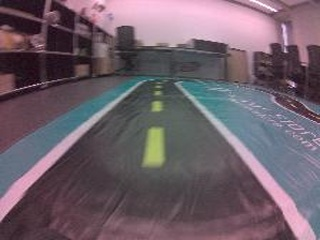
\includegraphics[width=1\textwidth]{experiments/0_.jpg}
	      \caption{Real image}\label{fig:real}
	  \end{subfigure}%
      \hfill
  \begin{subfigure}{.33\linewidth}
	      \centering
	      \scalebox{-1}[1]{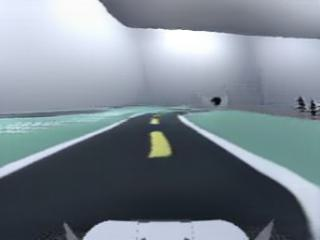
\includegraphics[width=1\textwidth]{experiments/0__.jpg}}
	      \caption{Pseudo-simulated image}\label{fig:psim}
	  \end{subfigure}%
  \hfill
  \begin{subfigure}{.33\linewidth}
	    \centering
	    \scalebox{-1}[1]{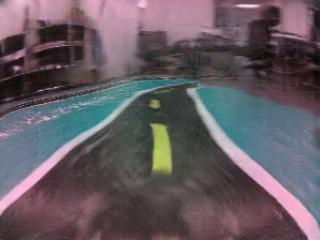
\includegraphics[width=1\textwidth]{experiments/0___.jpg}}
	    \caption{Pseudo-pseudo-real image}\label{fig:ppreal}
	  \end{subfigure} 
  \caption{Using the CycleGan to create a paired dateset}
  \label{fig:examplealigned}
\end{figure}

However, we can visually see that the quality of the translations degrades as more transformation steps are applied. Once obtained the paired dataset of authentic and pseudo images we computed the respective latent space vectors and used t-SNE to visualize them. The results are shown in Figure~\ref{fig:latentpseudoaligned}.

\begin{figure}[h]
  \centering
  \begin{subfigure}{.5\linewidth}
	      \centering
	      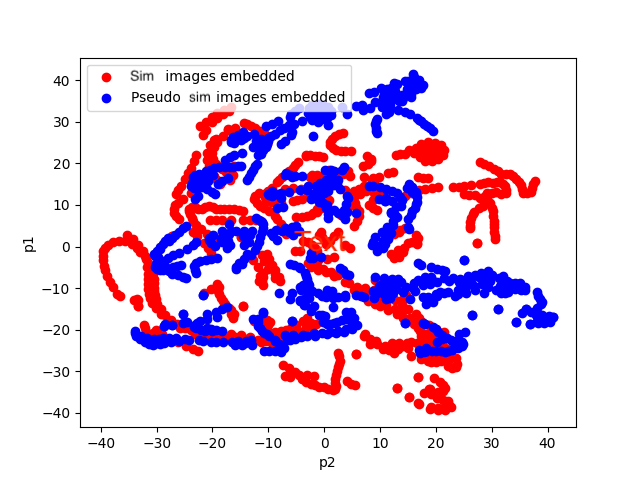
\includegraphics[width=1\textwidth]{experiments/aligned_latentr2s.png}
	      \caption{Paired Simulated (authentic) and pseudo-simulated images. \matteo{check labels}}\label{fig:aligen_latentr2s}
	  \end{subfigure}%
      \hfill
  \begin{subfigure}{.5\linewidth}
	      \centering
	      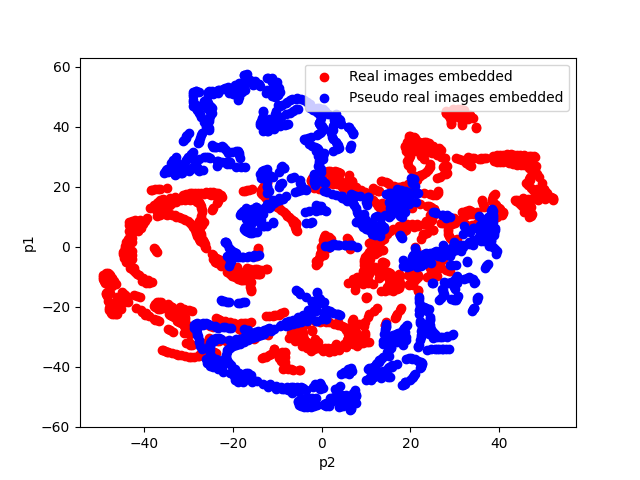
\includegraphics[width=1\textwidth]{experiments/aligned_latents2r.png}
	      \caption{Paired Real (authentic) and pseudo-real images.}\label{fig:aligen_latents2r}
	  \end{subfigure}
  \caption{Latent space visualization for the paired datasets: authentic vs pseudo (i.e., translated) images. (Left) simulated VAE, (right) real VAE.}
  \label{fig:latentpseudoaligned}
\end{figure}

However, the overlap of the embeddings does not seem to increase w.r.t. the unpaired datasets. We further proceeded with a more fine-grained analysis by looking at the single images in the datasets. In particular, considering the paired datasets, we randomly sampled pseudo images and computed their latent space representation. Then, we computed the Euclidean distance between such representation and all latent space representations in the authentic paired dataset and took the corresponding image whose latent space is the closest. Examples of such images are in Figure~\ref{fig:simdistance} for the simulated environment and in Figure~\ref{fig:realdistance}.

%Unfortunately, the results do not change enough from the previous one as shown in Figure \ref{fig:latentpseudoaligned}. Given that the t-SNEe dimensionality reduction may be a cause of our problem, a further investigation is made by checking what are the closest images between the real set and pseudo real set and similarly for the simulated set in the latent space. The distance measure used is the Euclidean distance and by looking at them there is some problem, in fact there are perfect matches as well as wrong matches as shown in Figures \ref{fig:simdistance} and \ref{fig:realdistance}. This may be the cause of our agent not being able to drive when transferred into another domain, the encoder is not robust enough to compensate little image distortion.

\begin{figure}[h]
  \centering
  \begin{subfigure}{.24\linewidth}
	      \centering
	      \scalebox{-1}[1]{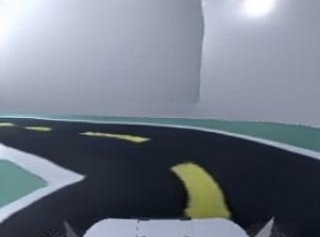
\includegraphics[width=1\textwidth]{experiments/badsimdist1.jpg}}
	      \caption{Pseudo simulated (Bad)}\label{fig:badsimdist1}
	  \end{subfigure}%
  \hfill
  \begin{subfigure}{.24\linewidth}
	    \centering
	    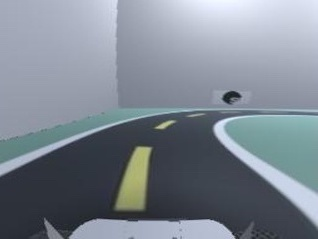
\includegraphics[width=1\textwidth]{experiments/badsimdist2.jpg}
	    \caption{Closest simulated (Bad)}\label{fig:badsimdist2}
	  \end{subfigure}%
  \hfill
  \begin{subfigure}{.24\linewidth}
	      \centering
	      \scalebox{-1}[1]{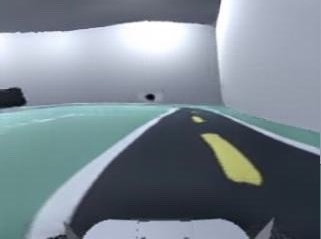
\includegraphics[width=1\textwidth]{experiments/goodsimdist1.jpg}}
	      \caption{Pseudo simulated (Good)}\label{fig:goodsimdist1}
	  \end{subfigure}%
  \hfill
  \begin{subfigure}{.24\linewidth}
	    \centering
	    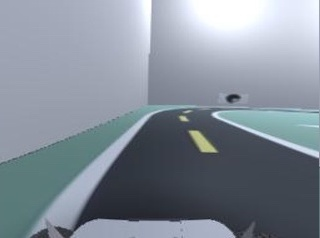
\includegraphics[width=1\textwidth]{experiments/goodsimdist2.jpg}
	    \caption{Closest simulated (Good)}\label{fig:goodsimdist2}
	\end{subfigure}
	  \caption{Figure~\ref{fig:badsimdist1} and Figure~\ref{fig:goodsimdist1} show two pseudo-simulated images. Respectively, Figure~\ref{fig:badsimdist2} and Figure~\ref{fig:goodsimdist2} are the closest match in the simulated set according to the Euclidean distance in the latent space of the simulated VAE.}
	  \label{fig:simdistance}
\end{figure}


\begin{figure}[h]
  \centering
  \begin{subfigure}{.24\linewidth}
	      \centering
	      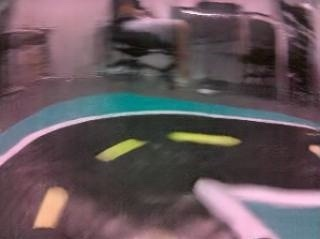
\includegraphics[width=1\textwidth]{experiments/badrealreal1.jpg}
	      \caption{Pseudo real (Bad)}\label{fig:badrealdist1}
	  \end{subfigure}%
  \hfill
  \begin{subfigure}{.24\linewidth}
	    \centering
	    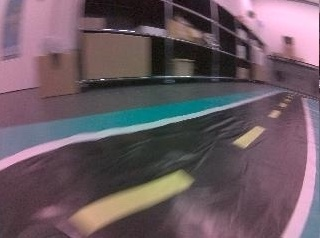
\includegraphics[width=1\textwidth]{experiments/badrealreal2.jpg}
	    \caption{Closest real (Bad)}\label{fig:badrealdist2}
	  \end{subfigure}%
  \hfill
  \begin{subfigure}{.24\linewidth}
	      \centering
	      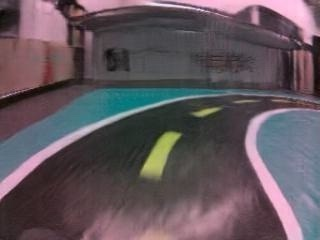
\includegraphics[width=1\textwidth]{experiments/goodrealdist1.jpg}
	      \caption{Pseudo real (Good)}\label{fig:goodrealdist1}
	  \end{subfigure}%
  \hfill
  \begin{subfigure}{.24\linewidth}
	    \centering
	    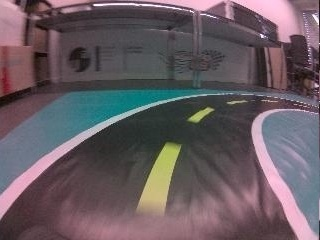
\includegraphics[width=1\textwidth]{experiments/goodrealdist2.jpg}
	    \caption{Closest real (Good)}\label{fig:goodrealdist2}
	\end{subfigure}
	  \caption{Figure~\ref{fig:badrealdist1} and Figure~\ref{fig:goodrealdist1} show two pseudo-real images. Respectively, Figure~\ref{fig:badrealdist2} and Figure~\ref{fig:goodrealdist2}, show the closest match in the real set according to the Euclidean distance in the latent space of the real VAE.}
	  \label{fig:realdistance}
\end{figure}

We can see from the images that in some cases the closest image in the latent space is actually similar to the authentic counterpart (see Good examples). On the other hand, there are also examples in critical parts of the track (see Figure~\ref{fig:badsimdist1} and Figure~\ref{fig:badrealdist1}), in which the closest authentic image in the latent space does not actually represent what is in the pseudo counterpart. As a consequence, transferring a trained agent from one domain into the other by using image-to-image translation seems challenging, as the VAE that represents the state for the trained policy does not seem to be robust w.r.t. the translations.

Finally, we analyzed the offline predictions of the agent we trained in the real world and compute the error between the prediction made by the agent when given the authentic real image and the prediction made when given the pseudo-real image. Specifically, we selected a set of 100 contiguous images from the real dataset and computed the corresponding paired translation, i.e. from real to simulated and from simulated to real \matteo{images of which sector of the track? Moreover, 100 images correspond to 5 seconds of simulation}. Then, we computed the prediction, i.e. the steering angle, of the trained agent when given each of the two images and plotted the results in Figure~\ref{fig:path_rec}. From the plot we can see that, most of the time, the predictions are aligned. The average prediction error is 0.205 with a standard deviation of 0.183. However, small prediction errors can accumulate over time leading the car in sectors of the track where it is not able to recover.

%As a final test, we are interested in studying what would be the actions undertaken by the agent on a set of aligned pictures. In particular, we selected a small set of 100 contiguous real pictures of the track and created its \textit{aligned} pseudo real version. We then checked what would be the action of the real agent. As shown in Figure \ref{fig:path_rec}, the results are interesting since most of the times the agent takes the same action on both images, however even a tiny difference can lead the car out of track from which often it is not able to recover. The mean error on the predicted action resulted to be 0.20 
%TODO INSERIRE STD E BREVE CONCLUSIONE DELLA SEZIONE 

\begin{figure}[h]
  \begin{center}
	    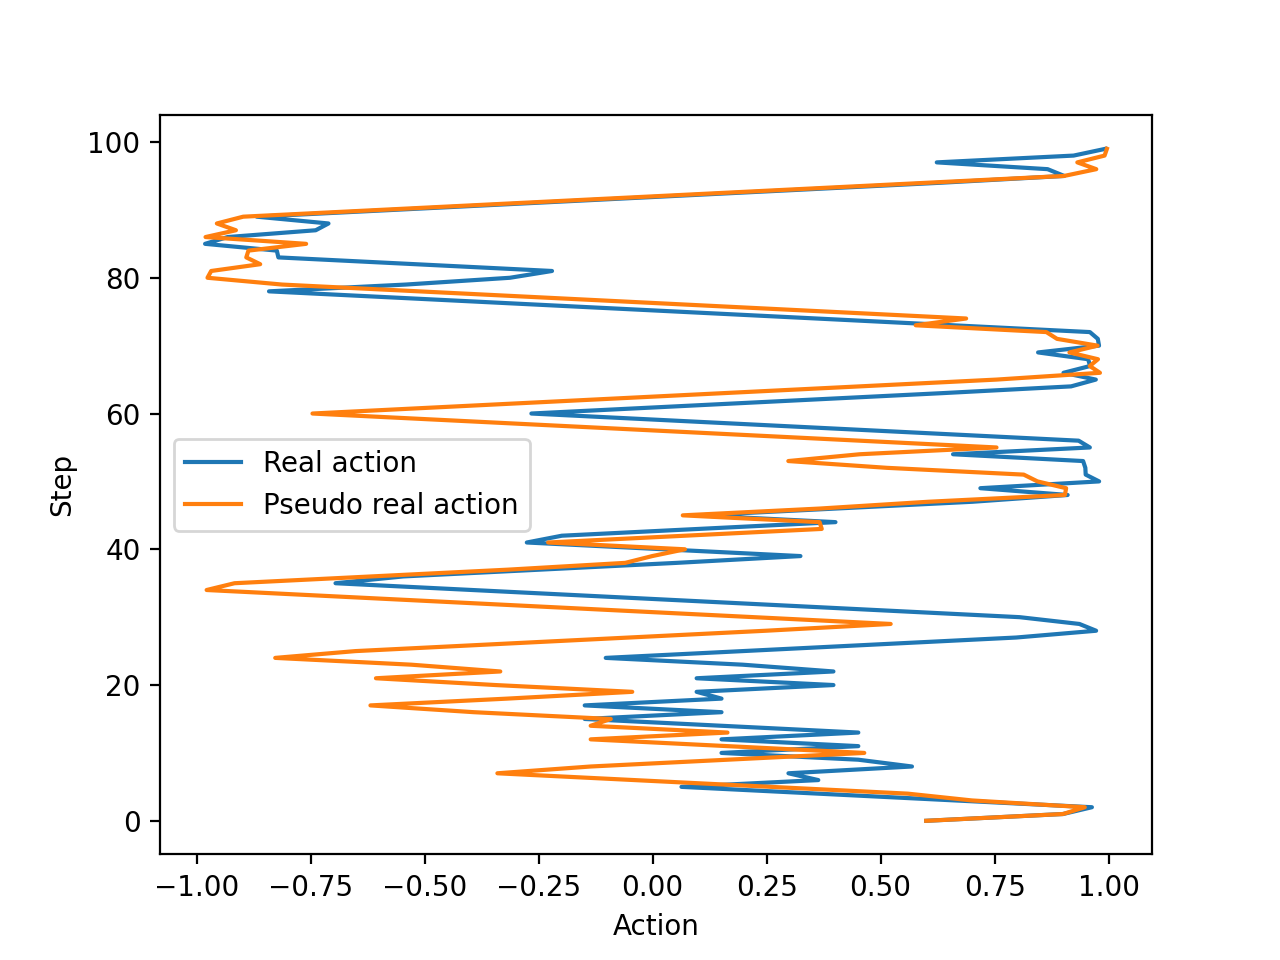
\includegraphics[width=0.60\textwidth]{experiments/path_rec.png}
	  \end{center}
  \caption{Trained agent predictions when given authentic real image and pseudo-real image.}
  \label{fig:path_rec}
\end{figure}

%\begin{figure}[h]
%  \begin{center}
	%    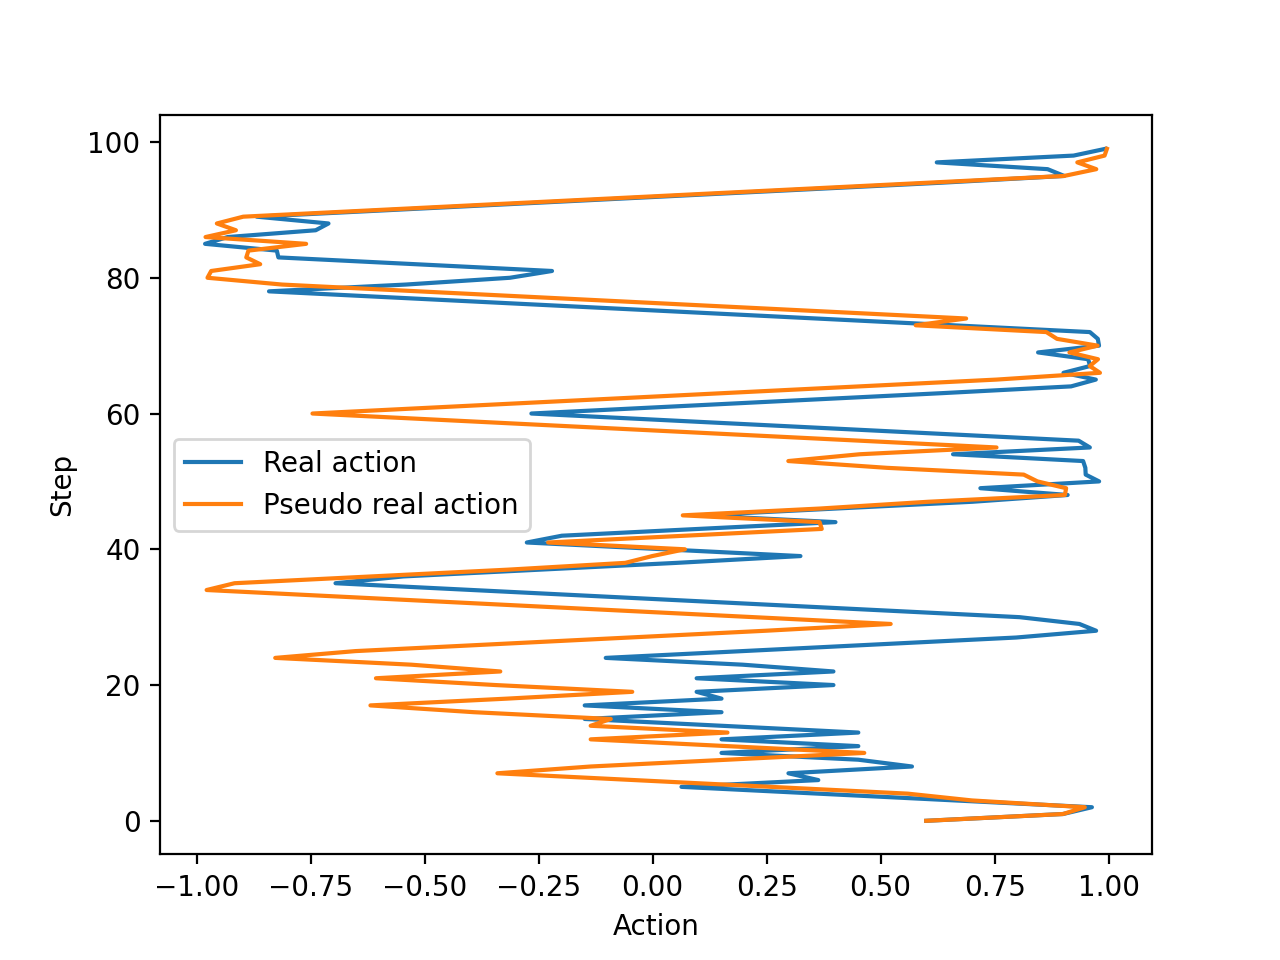
\includegraphics[width=0.60\textwidth]{experiments/path_rec.png}
	%  \end{center}
%  \caption{Real agent's actions on an aligned dataset}
%  \label{fig:path_rec}
%\end{figure}

%\begin{figure}[h]
%  \centering
%  \begin{subfigure}{.24\linewidth}
	%      \centering
	%      \scalebox{-1}[1]{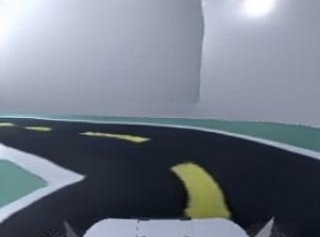
\includegraphics[width=1\textwidth]{experiments/badsimdist1.jpg}}
	%      \caption{Pseudo simulated}\label{fig:badsimdist1}
	%  \end{subfigure}%
%  \hfill
%  \begin{subfigure}{.24\linewidth}
	%    \centering
	%    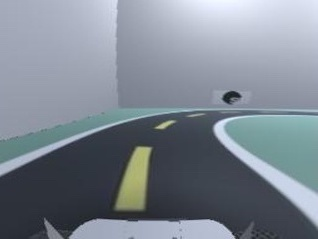
\includegraphics[width=1\textwidth]{experiments/badsimdist2.jpg}
	%    \caption{Closest simulated}\label{fig:badsimdist2}
	%  \end{subfigure}%
%  \hfill
%  \begin{subfigure}{.24\linewidth}
	%      \centering
	%      \scalebox{-1}[1]{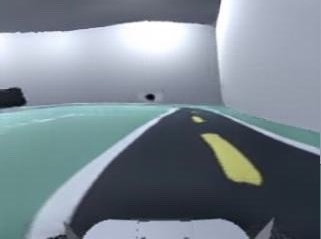
\includegraphics[width=1\textwidth]{experiments/goodsimdist1.jpg}}
	%      \caption{Pseudo simulated}\label{fig:goodsimdist1}
	%  \end{subfigure}%
%  \hfill
%  \begin{subfigure}{.24\linewidth}
%    \centering
%    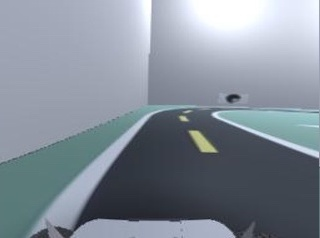
\includegraphics[width=1\textwidth]{experiments/goodsimdist2.jpg}
%    \caption{Closest simulated}\label{fig:goodsimdist2}
%\end{subfigure}
%  \caption{Figures \ref{fig:badsimdist1} and \ref{fig:goodsimdist1} show two pseudo simulated images and Figures \ref{fig:badsimdist2} and \ref{fig:goodsimdist2} respectively the closest match in the simulated set measured with the Euclidean Distance.}
%  \label{fig:simdistance}
%\end{figure}

%\begin{figure}[h]
%  \centering
%  \begin{subfigure}{.24\linewidth}
	%      \centering
	%      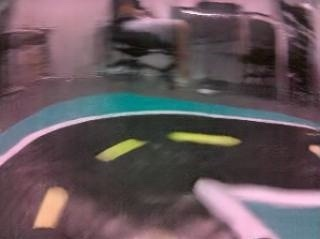
\includegraphics[width=1\textwidth]{experiments/badrealreal1.jpg}
	%      \caption{Pseudo real}\label{fig:badrealdist1}
	%  \end{subfigure}%
%  \hfill
%  \begin{subfigure}{.24\linewidth}
	%    \centering
	%    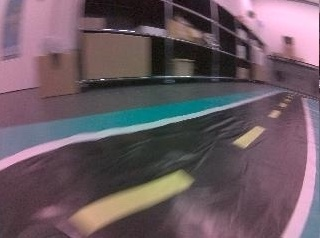
\includegraphics[width=1\textwidth]{experiments/badrealreal2.jpg}
	%    \caption{Closest real}\label{fig:badrealdist2}
	%  \end{subfigure}%
%  \hfill
%  \begin{subfigure}{.24\linewidth}
	%      \centering
	%      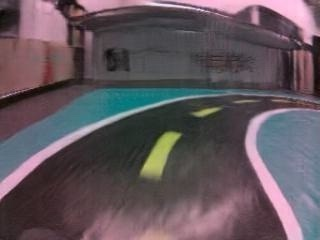
\includegraphics[width=1\textwidth]{experiments/goodrealdist1.jpg}
	%      \caption{Pseudo real}\label{fig:goodrealdist1}
	%  \end{subfigure}%
%  \hfill
%  \begin{subfigure}{.24\linewidth}
	%    \centering
	%    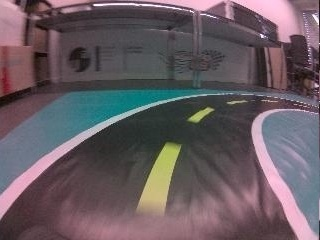
\includegraphics[width=1\textwidth]{experiments/goodrealdist2.jpg}
	%    \caption{Closest real}\label{fig:goodrealdist2}
	%\end{subfigure}
	%  \caption{Figures \ref{fig:badrealdist1} and \ref{fig:goodrealdist1} show two pseudo real images and Figures \ref{fig:badrealdist2} and \ref{fig:goodrealdist2} respectively the closest match in the real set measured with the Euclidean Distance.}
	%  \label{fig:realdistance}
	%\end{figure}


%Unfortunately, the results do not change enough from the previous one as shown in Figure \ref{fig:latentpseudoaligned}. Given that the t-SNEe dimensionality reduction may be a cause of our problem, a further investigation is made by checking what are the closest images between the real set and pseudo real set and similarly for the simulated set in the latent space. The distance measure used is the Euclidean distance and by looking at them there is some problem, in fact there are perfect matches as well as wrong matches as shown in Figures \ref{fig:simdistance} and \ref{fig:realdistance}. This may be the cause of our agent not being able to drive when transferred into another domain, the encoder is not robust enough to compensate little image distortion.


%Hence, the real test set is transformed through the CycleGAN and then forwarded through the real VAE chosen and similarly for the simulated test set. Given that 64 dimension cannot be visualized, a further dimensionality reduction is applied with t-SNE down to two dimension, as shown in Figure \ref{fig:latentpseudo}.
%
%\begin{figure}[h]
%  \centering
%  \begin{subfigure}{.5\linewidth}
%      \centering
%      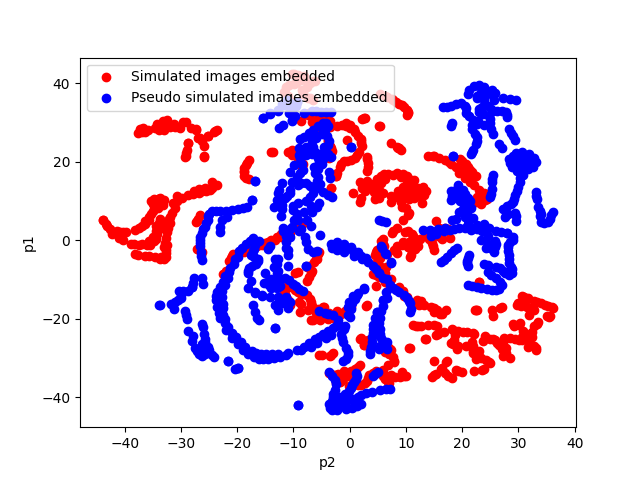
\includegraphics[width=1\textwidth]{experiments/latentr2s.png}
%      \caption{Simulated and pseudo simulated images}\label{fig:latentr2s}
%  \end{subfigure}%
%      \hfill
%  \begin{subfigure}{.5\linewidth}
%      \centering
%      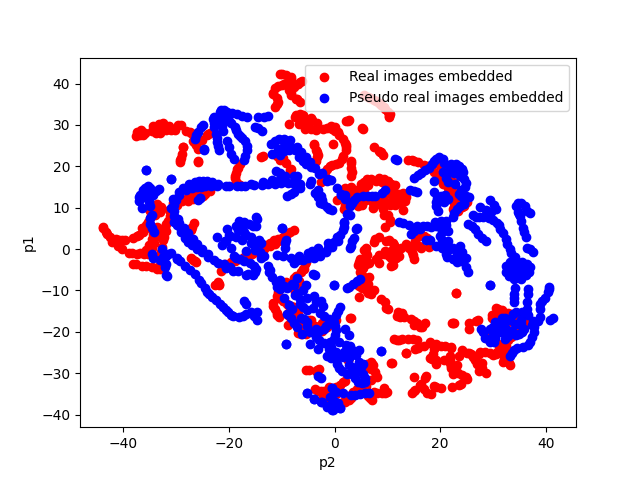
\includegraphics[width=1\textwidth]{experiments/latents2r.png}
%      \caption{Real and pseudo real images}\label{fig:latents2r}
%  \end{subfigure}
%  \caption{Images embedded into the latent space with respectively the simulated and the real VAE.}
%  \label{fig:latentpseudo}
%\end{figure}
%Since the datasets are not aligned we do not except a perfect overlap, instead, the encoder should be able to at least embed similar images in the same region of the space. However, the latent space shows that is not always the case, some regions does overlap but not all off them in both real and simulated dataset. This could lead the trained agent not to respond consistently in similar situations. A further attempt is made by aligning the set of data used through the CycleGAN. Once the CycleGAN has been used to transform simulated images into pseudo real images, it can be used again to bring them back to pseudo simulated images, resulting in aligned sets. However, notice that the distortion, barely visible before, increases as shown in Figure \ref{fig:examplealigned}.
%
%\begin{figure}[h]
%  \centering
%  \begin{subfigure}{.33\linewidth}
%      \centering
%      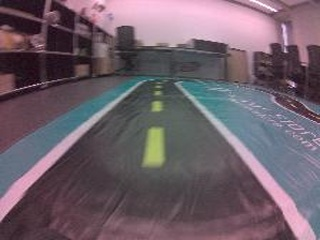
\includegraphics[width=1\textwidth]{experiments/0_.jpg}
%      \caption{Real image}\label{fig:real}
%  \end{subfigure}%
%      \hfill
%  \begin{subfigure}{.33\linewidth}
%      \centering
%      \scalebox{-1}[1]{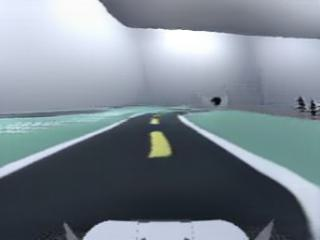
\includegraphics[width=1\textwidth]{experiments/0__.jpg}}
%      \caption{Pseudo simulated image}\label{fig:psim}
%  \end{subfigure}%
%  \hfill
%  \begin{subfigure}{.33\linewidth}
%    \centering
%    \scalebox{-1}[1]{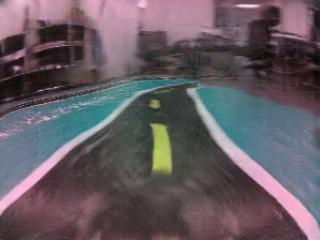
\includegraphics[width=1\textwidth]{experiments/0___.jpg}}
%    \caption{Pseudo pseudo real}\label{fig:ppreal}
%  \end{subfigure} 
%  \caption{Example of using the CycleGan to create an aligned dateset}
%  \label{fig:examplealigned}
%\end{figure}
%
%\begin{figure}[h]
%  \centering
%  \begin{subfigure}{.5\linewidth}
%      \centering
%      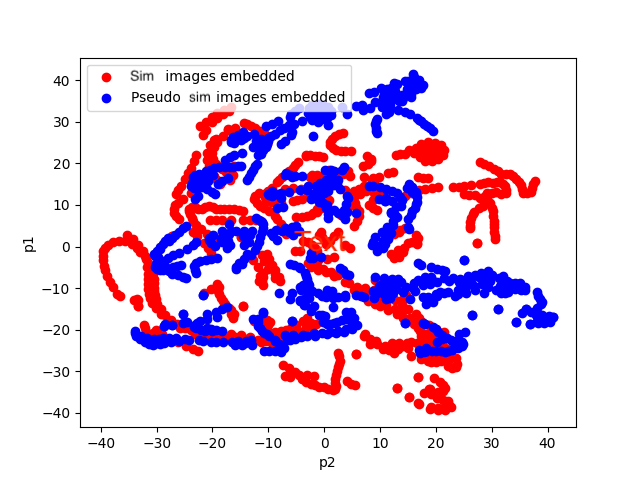
\includegraphics[width=1\textwidth]{experiments/aligned_latentr2s.png}
%      \caption{Aligned simulated and pseudo sim images}\label{fig:aligen_latentr2s}
%  \end{subfigure}%
%      \hfill
%  \begin{subfigure}{.5\linewidth}
%      \centering
%      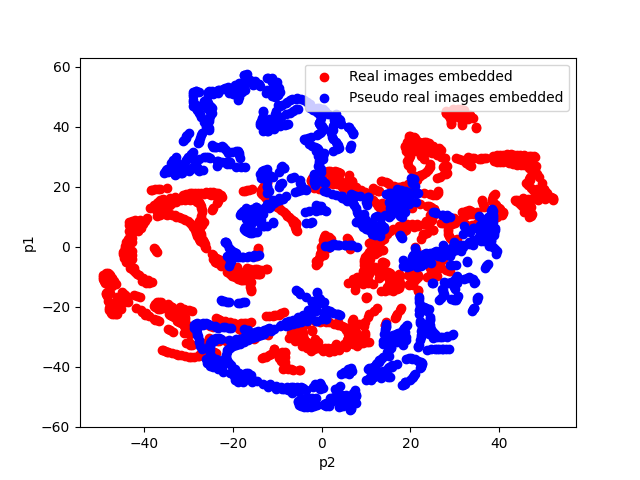
\includegraphics[width=1\textwidth]{experiments/aligned_latents2r.png}
%      \caption{Aligned real and pseudo real images}\label{fig:aligen_latents2r}
%  \end{subfigure}
%  \caption{Aligned images embedded into the latent space with respectively the simulated and the real VAE.}
%  \label{fig:latentpseudoaligned}
%\end{figure}
%
%Unfortunately, the results do not change enough from the previous one as shown in Figure \ref{fig:latentpseudoaligned}. Given that the t-SNEe dimensionality reduction may be a cause of our problem, a further investigation is made by checking what are the closest images between the real set and pseudo real set and similarly for the simulated set in the latent space. The distance measure used is the Euclidean distance and by looking at them there is some problem, in fact there are perfect matches as well as wrong matches as shown in Figures \ref{fig:simdistance} and \ref{fig:realdistance}. This may be the cause of our agent not being able to drive when transferred into another domain, the encoder is not robust enough to compensate little image distortion.
%
%As a final test, we are interested in studying what would be the actions undertaken by the agent on a set of aligned pictures. In particular, we selected a small set of 100 contiguous real pictures of the track and created its \textit{aligned} pseudo real version. We then checked what would be the action of the real agent. As shown in Figure \ref{fig:path_rec}, the results are interesting since most of the times the agent takes the same action on both images, however even a tiny difference can lead the car out of track from which often it is not able to recover. The mean error on the predicted action resulted to be 0.20 
%TODO INSERIRE STD E BREVE CONCLUSIONE DELLA SEZIONE 
%
%\begin{figure}[h]
%  \begin{center}
%    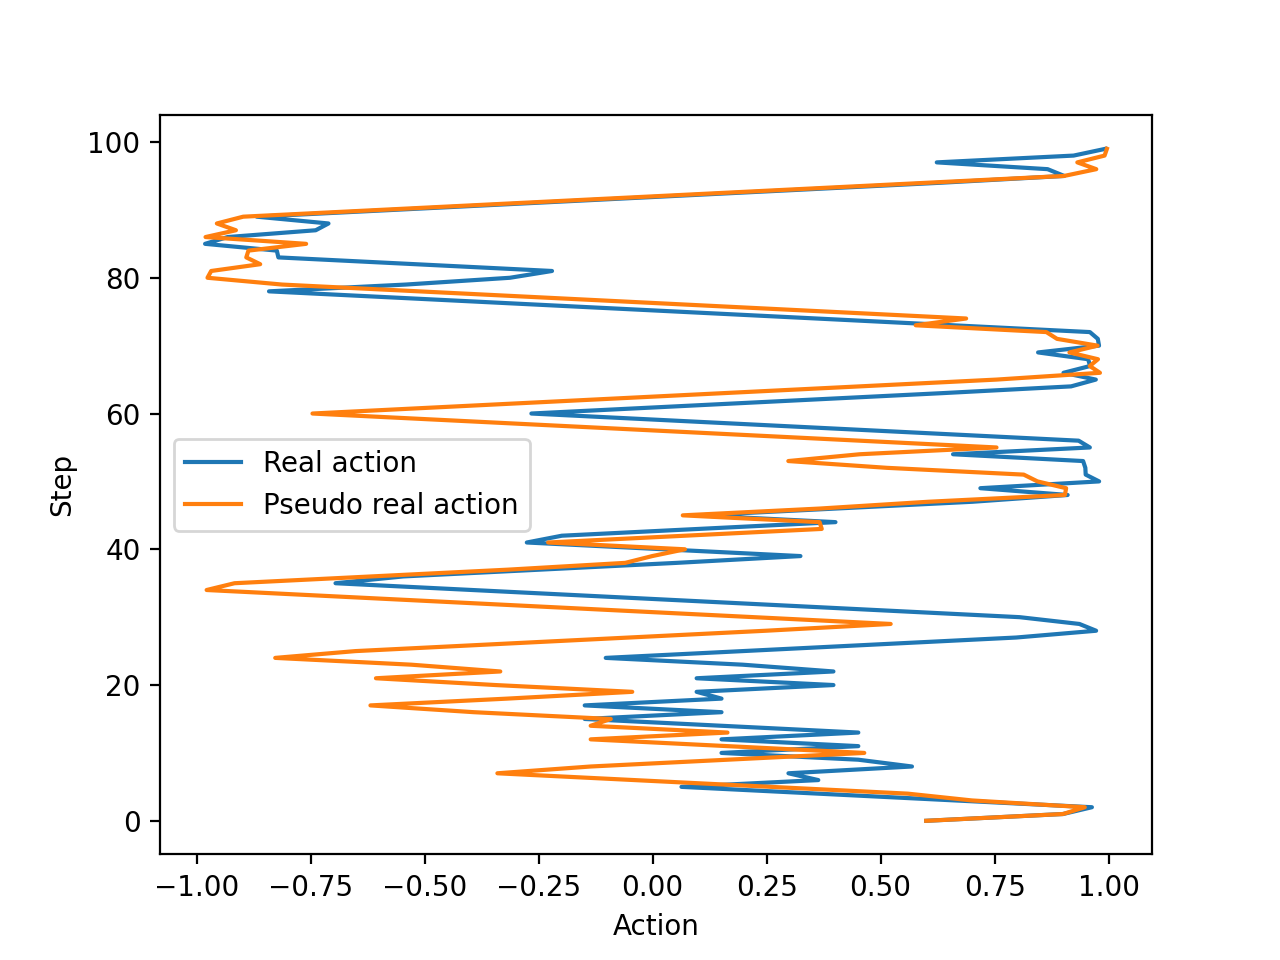
\includegraphics[width=0.60\textwidth]{experiments/path_rec.png}
%  \end{center}
%  \caption{Real agent's actions on an aligned dataset}
%  \label{fig:path_rec}
%\end{figure}
%
%\begin{figure}[h]
%  \centering
%  \begin{subfigure}{.24\linewidth}
%      \centering
%      \scalebox{-1}[1]{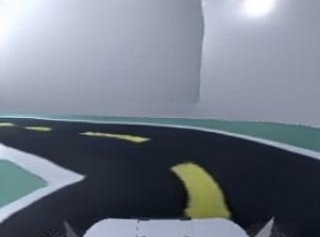
\includegraphics[width=1\textwidth]{experiments/badsimdist1.jpg}}
%      \caption{Pseudo simulated}\label{fig:badsimdist1}
%  \end{subfigure}%
%  \hfill
%  \begin{subfigure}{.24\linewidth}
%    \centering
%    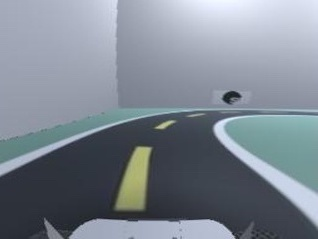
\includegraphics[width=1\textwidth]{experiments/badsimdist2.jpg}
%    \caption{Closest simulated}\label{fig:badsimdist2}
%  \end{subfigure}%
%  \hfill
%  \begin{subfigure}{.24\linewidth}
%      \centering
%      \scalebox{-1}[1]{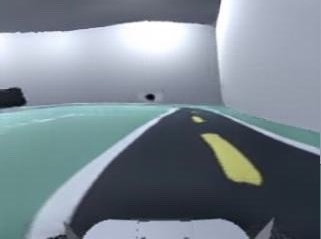
\includegraphics[width=1\textwidth]{experiments/goodsimdist1.jpg}}
%      \caption{Pseudo simulated}\label{fig:goodsimdist1}
%  \end{subfigure}%
%  \hfill
%  \begin{subfigure}{.24\linewidth}
%    \centering
%    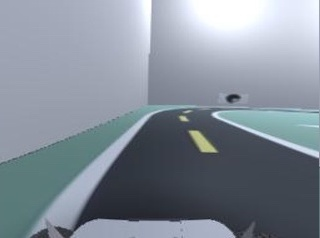
\includegraphics[width=1\textwidth]{experiments/goodsimdist2.jpg}
%    \caption{Closest simulated}\label{fig:goodsimdist2}
%\end{subfigure}
%  \caption{Figures \ref{fig:badsimdist1} and \ref{fig:goodsimdist1} show two pseudo simulated images and Figures \ref{fig:badsimdist2} and \ref{fig:goodsimdist2} respectively the closest match in the simulated set measured with the Euclidean Distance.}
%  \label{fig:simdistance}
%\end{figure}
%
%\begin{figure}[h]
%  \centering
%  \begin{subfigure}{.24\linewidth}
%      \centering
%      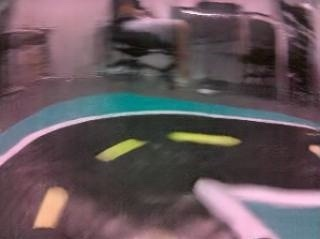
\includegraphics[width=1\textwidth]{experiments/badrealreal1.jpg}
%      \caption{Pseudo real}\label{fig:badrealdist1}
%  \end{subfigure}%
%  \hfill
%  \begin{subfigure}{.24\linewidth}
%    \centering
%    \includegraphics[width=1\textwidth]{experiments/badrealreal2.jpg}
%    \caption{Closest real}\label{fig:badrealdist2}
%  \end{subfigure}%
%  \hfill
%  \begin{subfigure}{.24\linewidth}
%      \centering
%      \includegraphics[width=1\textwidth]{experiments/goodrealdist1.jpg}
%      \caption{Pseudo real}\label{fig:goodrealdist1}
%  \end{subfigure}%
%  \hfill
%  \begin{subfigure}{.24\linewidth}
%    \centering
%    \includegraphics[width=1\textwidth]{experiments/goodrealdist2.jpg}
%    \caption{Closest real}\label{fig:goodrealdist2}
%\end{subfigure}
%  \caption{Figures \ref{fig:badrealdist1} and \ref{fig:goodrealdist1} show two pseudo real images and Figures \ref{fig:badrealdist2} and \ref{fig:goodrealdist2} respectively the closest match in the real set measured with the Euclidean Distance.}
%  \label{fig:realdistance}
%\end{figure}



